\documentclass[12pt, a4paper]{report}
\usepackage{graphicx}
\usepackage[french]{babel}
\usepackage{url}
\usepackage[utf8]{inputenc}
\usepackage[T1]{fontenc}
\usepackage{amsmath}
\usepackage{tikz}
\usepackage{listings}
\usepackage{parskip}
\usepackage{fancyhdr}
\usepackage{vmargin}
\usepackage{algorithmic}
\usepackage[ruled,vlined]{algorithm2e}
\usepackage{amsfonts}
\usepackage{amssymb}

\setmarginsrb{2 cm}{1.5 cm}{2 cm}{2.5 cm}{1 cm}{1 cm}{1 cm}{1.5 cm}
%1 est la marge gauche
%2 est la marge en haut
%3 est la marge droite
%4 est la marge en bas
%5 fixe la hauteur de l’entête
%6 fixe la distance entre l’entête et le texte
%7 fixe la hauteur du pied de page
%8 fixe la distance entre le texte et le pied de page
\author{Elias Bendjaballah}
\date{today's date}


\begin{document}

\begin{titlepage}

\centering

\includegraphics[scale=0.75]{logo2.png}
\par\vspace{1cm}
\vspace{1cm}
{\scshape\large\textbf{Projet LU3IN003} \par}
\vspace{1.5cm}
\rule{\linewidth}{0.2 mm}
{\huge\bfseries Alignement de séquences \par}
\rule{\linewidth}{0.2 mm}
\par\vspace{2cm}
{\scshape\large\itshape  Dao Quoc Hiep , Elias Bendjaballah \par}
\vfill
\large\textsc{Rapport}
\vfill
%Bas de page
{\large \today\par}

\end{titlepage}

%Optionnel
\tableofcontents
\pagebreak
%verifier à la fin

%Premier élément de la table des matières à 1 (pour l'index)
\renewcommand{\thesection}{\arabic{section}}
\section{Le problème d'alignement des séquences}
\subsection{Alignement de deux mots}
\subsubsection{Question 1}
On montre que si ($\overline{x} ,\overline{y}$) est un alignement de ($x,y$) et ($\overline{u},\overline{v}$) un alignement de ($u,v$) alors ($\overline{x}\cdot \overline{u},\overline{y} \cdot \overline{v}$) est un alignement de ($x\cdot u,y\cdot v$).\\
Par l'absurde, supposons que ($\overline{x} ,\overline{y}$) soit un alignement de ($x,y$) et ($\overline{u},\overline{v}$) un alignement de ($u,v$) et que ($\overline{x}\cdot \overline{u},\overline{y} \cdot \overline{v}$) ne soit pas un alignement de ($x\cdot u,y\cdot v$). Alors, il existerait au moins un déséquencement dans ($\overline{x}\cdot \overline{u},\overline{y} \cdot \overline{v}$). Ce déséquencement peut alors se trouver dans l'un des sous-mots $\overline{x}$, $\overline{y}$, $\overline{u}$ ou $\overline{v}$. S'il se trouve dans $\overline{x}$ ou $\overline{y}$ alors (par définition d'un alignement et selon la condition (iii) $|\overline{x}|=|\overline{y}|$ ou n'importe quelle autre condition provoquant un déséquencement),  ($\overline{x} ,\overline{y}$) n'est pas un alignement de ($x,y$) ce qui est en contradiction avec l'hypothèse de départ.\\
De manière similaire, si le déséquencement se trouve dans $\overline{u}$ ou $\overline{v}$ alors ($\overline{u},\overline{v}$) n'est pas un alignement de ($u,v$) ce qui contredit l'hypothèse de départ.\\
On en déduit que si ($\overline{x} ,\overline{y}$) est un alignement de ($x,y$) et ($\overline{u},\overline{v}$) un alignement de ($u,v$) alors ($\overline{x}\cdot \overline{u},\overline{y} \cdot \overline{v}$) est un alignement de ($x\cdot u,y\cdot v$).

\subsubsection{Question 2}
La longueur maximale d'un alignement $(x,y)$ est de : $|x|+|y|$ soit une valeur de $n+m$.\\
Cette valeur correspond au cas où les déséquencements ne sont corrigés que par des insertions et des délétions.
Un exemple possible est :\\
Si l'on considère x=ATTAGCGTTA et y=AGCTCGATGA, on peut obtenir :
\begin{center}
\rule{0.9\textwidth}{.4pt}
\begin{tabular}{lllllllllllllllllllllllllllllll}
$\overline{x}$ :&A&T&T&A&G&C&G&T&T&A&-&-&-&-&-&-&-&-&-&-\\
$\overline{y}$ :&-&-&-&-&-&-&-&-&-&-&A&G&C&T&C&G&A&T&G&A&\\
\end{tabular}
\rule{0.9\textwidth}{.4pt}
\end{center}

\section{Algorithmes pour l'alignement de séquences }
\subsection{Méthode naïve par énumération}


\subsubsection{Question 3}
Le nombre de mots de longueur n pouvant être obtenus en ajoutant exactement k gaps est donné par :
$$\binom{n+k}{k}=C_{n+k}^{k}=\frac{(n+k)!}{k!(n+k-k)!}=\frac{(n+k)!}{k! n!}$$
Il s'agit du nombre de manières possibles d'arranger les k gaps du mot $\overline{x}$ parmi les $n+k$ possibilités engendrées par ces insertions. 


\subsubsection{Question 4}
Sachant que $n \geq m$ et que $k$ gaps sont ajoutés à $x$ , on aura $k'=n-m+k$ gaps ajoutés à $y$. Avec $n-m$ les gaps à ajouter en raison de la possible différence de taille entre $x$ et $y$ et $k$ les gaps devant être ajoutés pour satisfaire le $(iii)$ de la définition d'un alignement ($|\overline{x}|=|\overline{y}|$).\\
Le nombre de manières possibles d'insérer ces gaps dans $y$, sachant qu'un gap de $\overline{y}$ ne doit pas être à la même position qu'un gap de $\overline{x}$ est donné par :
$$C_{n}^{k'}=\binom{n}{n-m+k}=\frac{n!}{(n-m+k)!(m-k)!}$$
On en déduit le nombre d'alignements possibles de ($x,y$):\\
Pour chaque k gap(s) ajoutés, il est possible d'obtenir $C_{n+k}^{k}$ versions de $x$ et pour chaque $x$, on peut obtenir $C_{n}^{k'}$  versions de $y$ donnant un alignement correct. Ce qui permet d'écrire :
$$A=\sum_{k=0}^{m}C_{n+k}^{k} \times C_{n}^{n-m+k}$$
$$A=\sum_{k=0}^{m}\frac{(n+k)!}{k! n!} \times \frac{n!}{(n-m+k)!(m-k)!}=\frac{(n+k)!}{k!(n-m+k)!(m-k)!}$$
Pour $|x|=15$ et $|y|=10$, on obtient un résultat de : 
$$A=\sum_{k=0}^{10}C_{15+k}^{k} \times C_{15}^{5+k}=298\ 199\ 265\  \text{alignements possibles.}$$

\subsubsection{Question 5}
Un algorithme naïf qui consisterait à énumérer tous les alignements de deux mots en vue de trouver la distance d'édition aurait une complexité exponentielle comme calculé à la question précédente. Il faudrait lister la totalité des alignements possibles pour ensuite retourner celui dont la distance d'édition est minimale.\\
$$\Theta (\sum_{k=0}^{m}\frac{(n+k)!}{k!(n-m+k)!(m-k)!}) \subset \mathcal{O}(n!)$$
Il en est de même pour un algorithme qui procéderait similairement pour retourner un alignement de coût minimal. Sa complexité serait aussi en $\mathcal{O}(n!)$.

\subsubsection{Question 6}
La complexité spatiale d'un algorithme naïf qui énumérerait tous les alignements de deux mots pour retourner la distance d'édition serait de $\mathcal{O}(n!)$ si on garde en mémoire à chaque étape et pour chaque possibilité, le coût total des modifications réalisées.\\
Un algorithme qui retournerait un alignement de coût minimal serait dans le pire cas (en considérant les alignements les plus longs possibles, soit ceux de taille $n+m$) :
$$\mathcal{O}(n!) \times 2(n+m) \text{ soit }\mathcal{O}(n!2(n+m)) \subset \mathcal{O}(n!)$$
On passe en $\mathcal{O}$ en raison du fait que ce cas n'est pas atteint.
\subsubsection{Tâche A}
\underline{Représentation du temps d'éxecution de DIST\_NAIF en fonction des instances testées :}\\
La première instance dont la résolution prend plus d'une minute est $Inst\_0000012\_56.adn$ avec une durée d'éxecution d'environ $293$ secondes. \\
\begin{center}
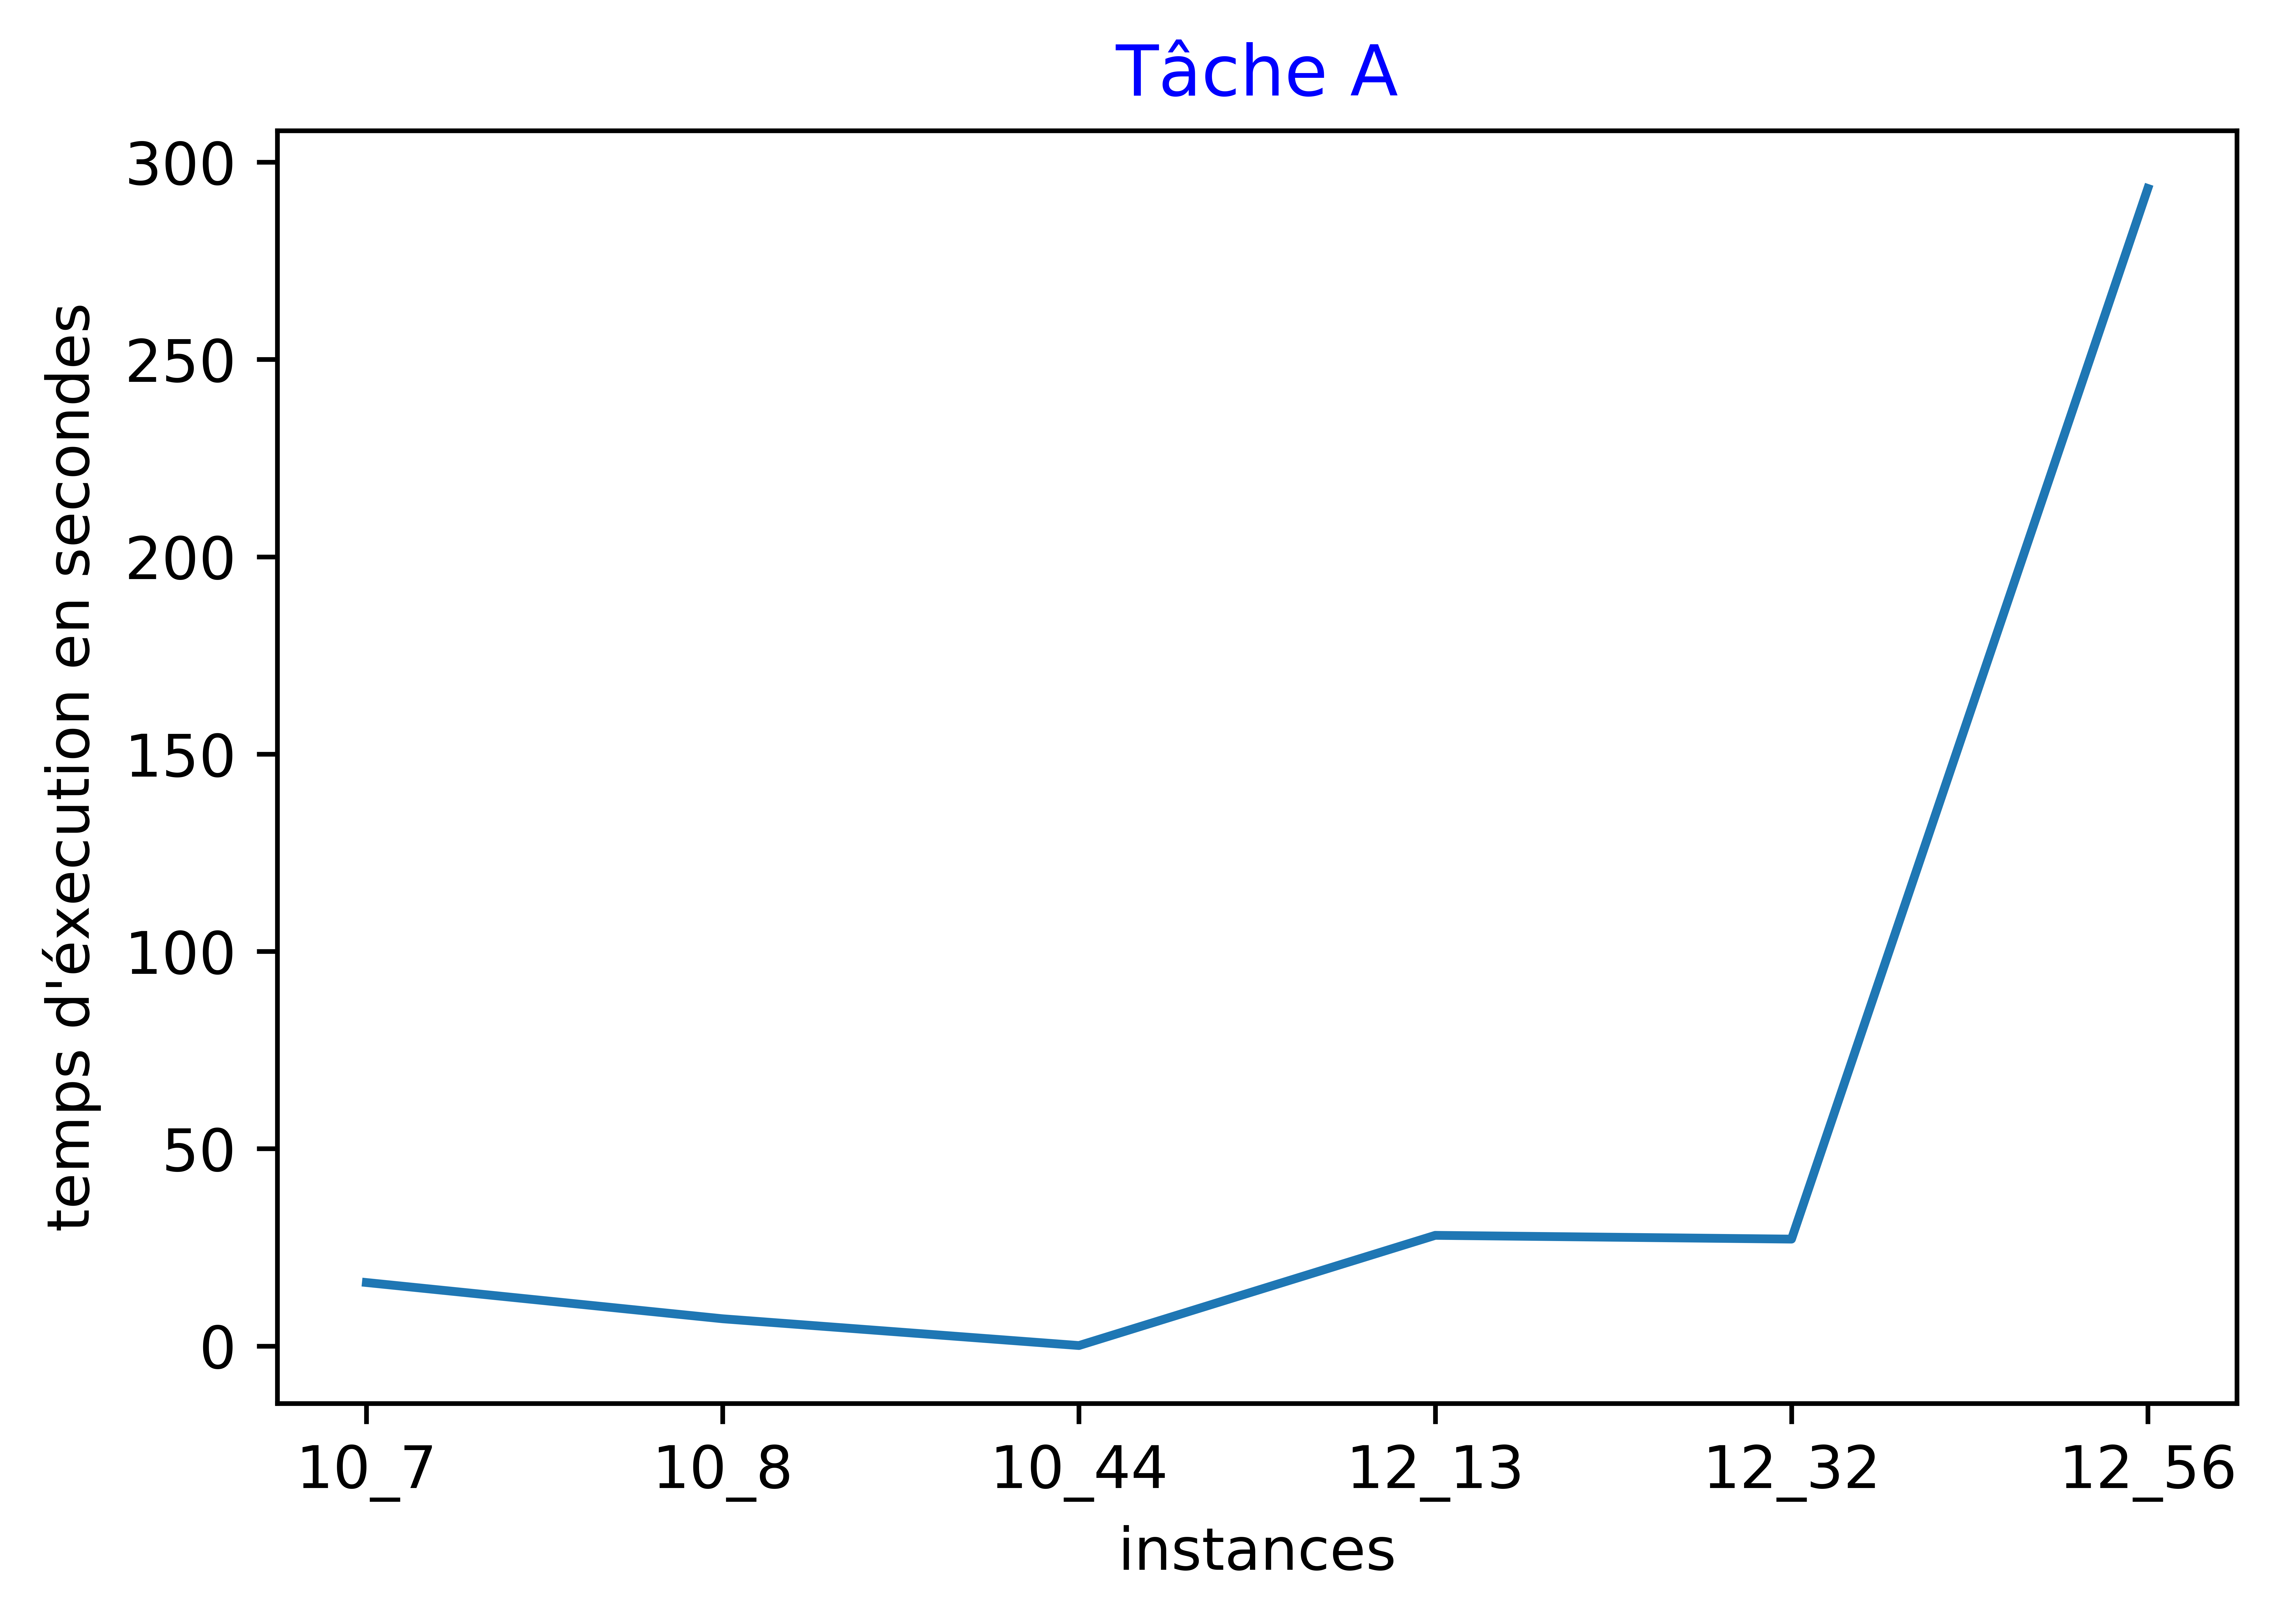
\includegraphics[scale=0.75]{TA.png}
\end{center}
L'évolution de la courbe avec une augmentation importante pour $Inst\_0000012\_56.adn$ où l'on a $|x|=12$ et $|y|=11$ suggère qu'il s'agit d'une fonction dont la complexité temporelle est exponentielle, ce qui est en accord avec le résultat de la question 5.\\Cette augmentation brutale peut s'expliquer par le nombre important de possibilités d'alignements de cette instance. En effet, pour $|x|=12$ et $|y|=11$, on peut avoir d'après la formule de la question 4, $A=103\ 274\ 625$ alignements possibles. Tandis que pour l'instance précédente $Inst\_0000012\_32.adn$, on a $|x|=12$ et $|y|=9$, ce qui engendre $A=14\ 218\ 905$ alignements possibles. Soit bien moins que $Inst\_0000012\_56.adn$, d'où la différence des temps d'éxecution des deux instances.\\
\underline{Représentation de la consommation mémoire de DIST\_NAIF en fonction des instances testées :}\\
Nous avons essayé de mesurer la consommation mémoire de la tâche A mais avons rencontré quelques difficultés.
\begin{center}
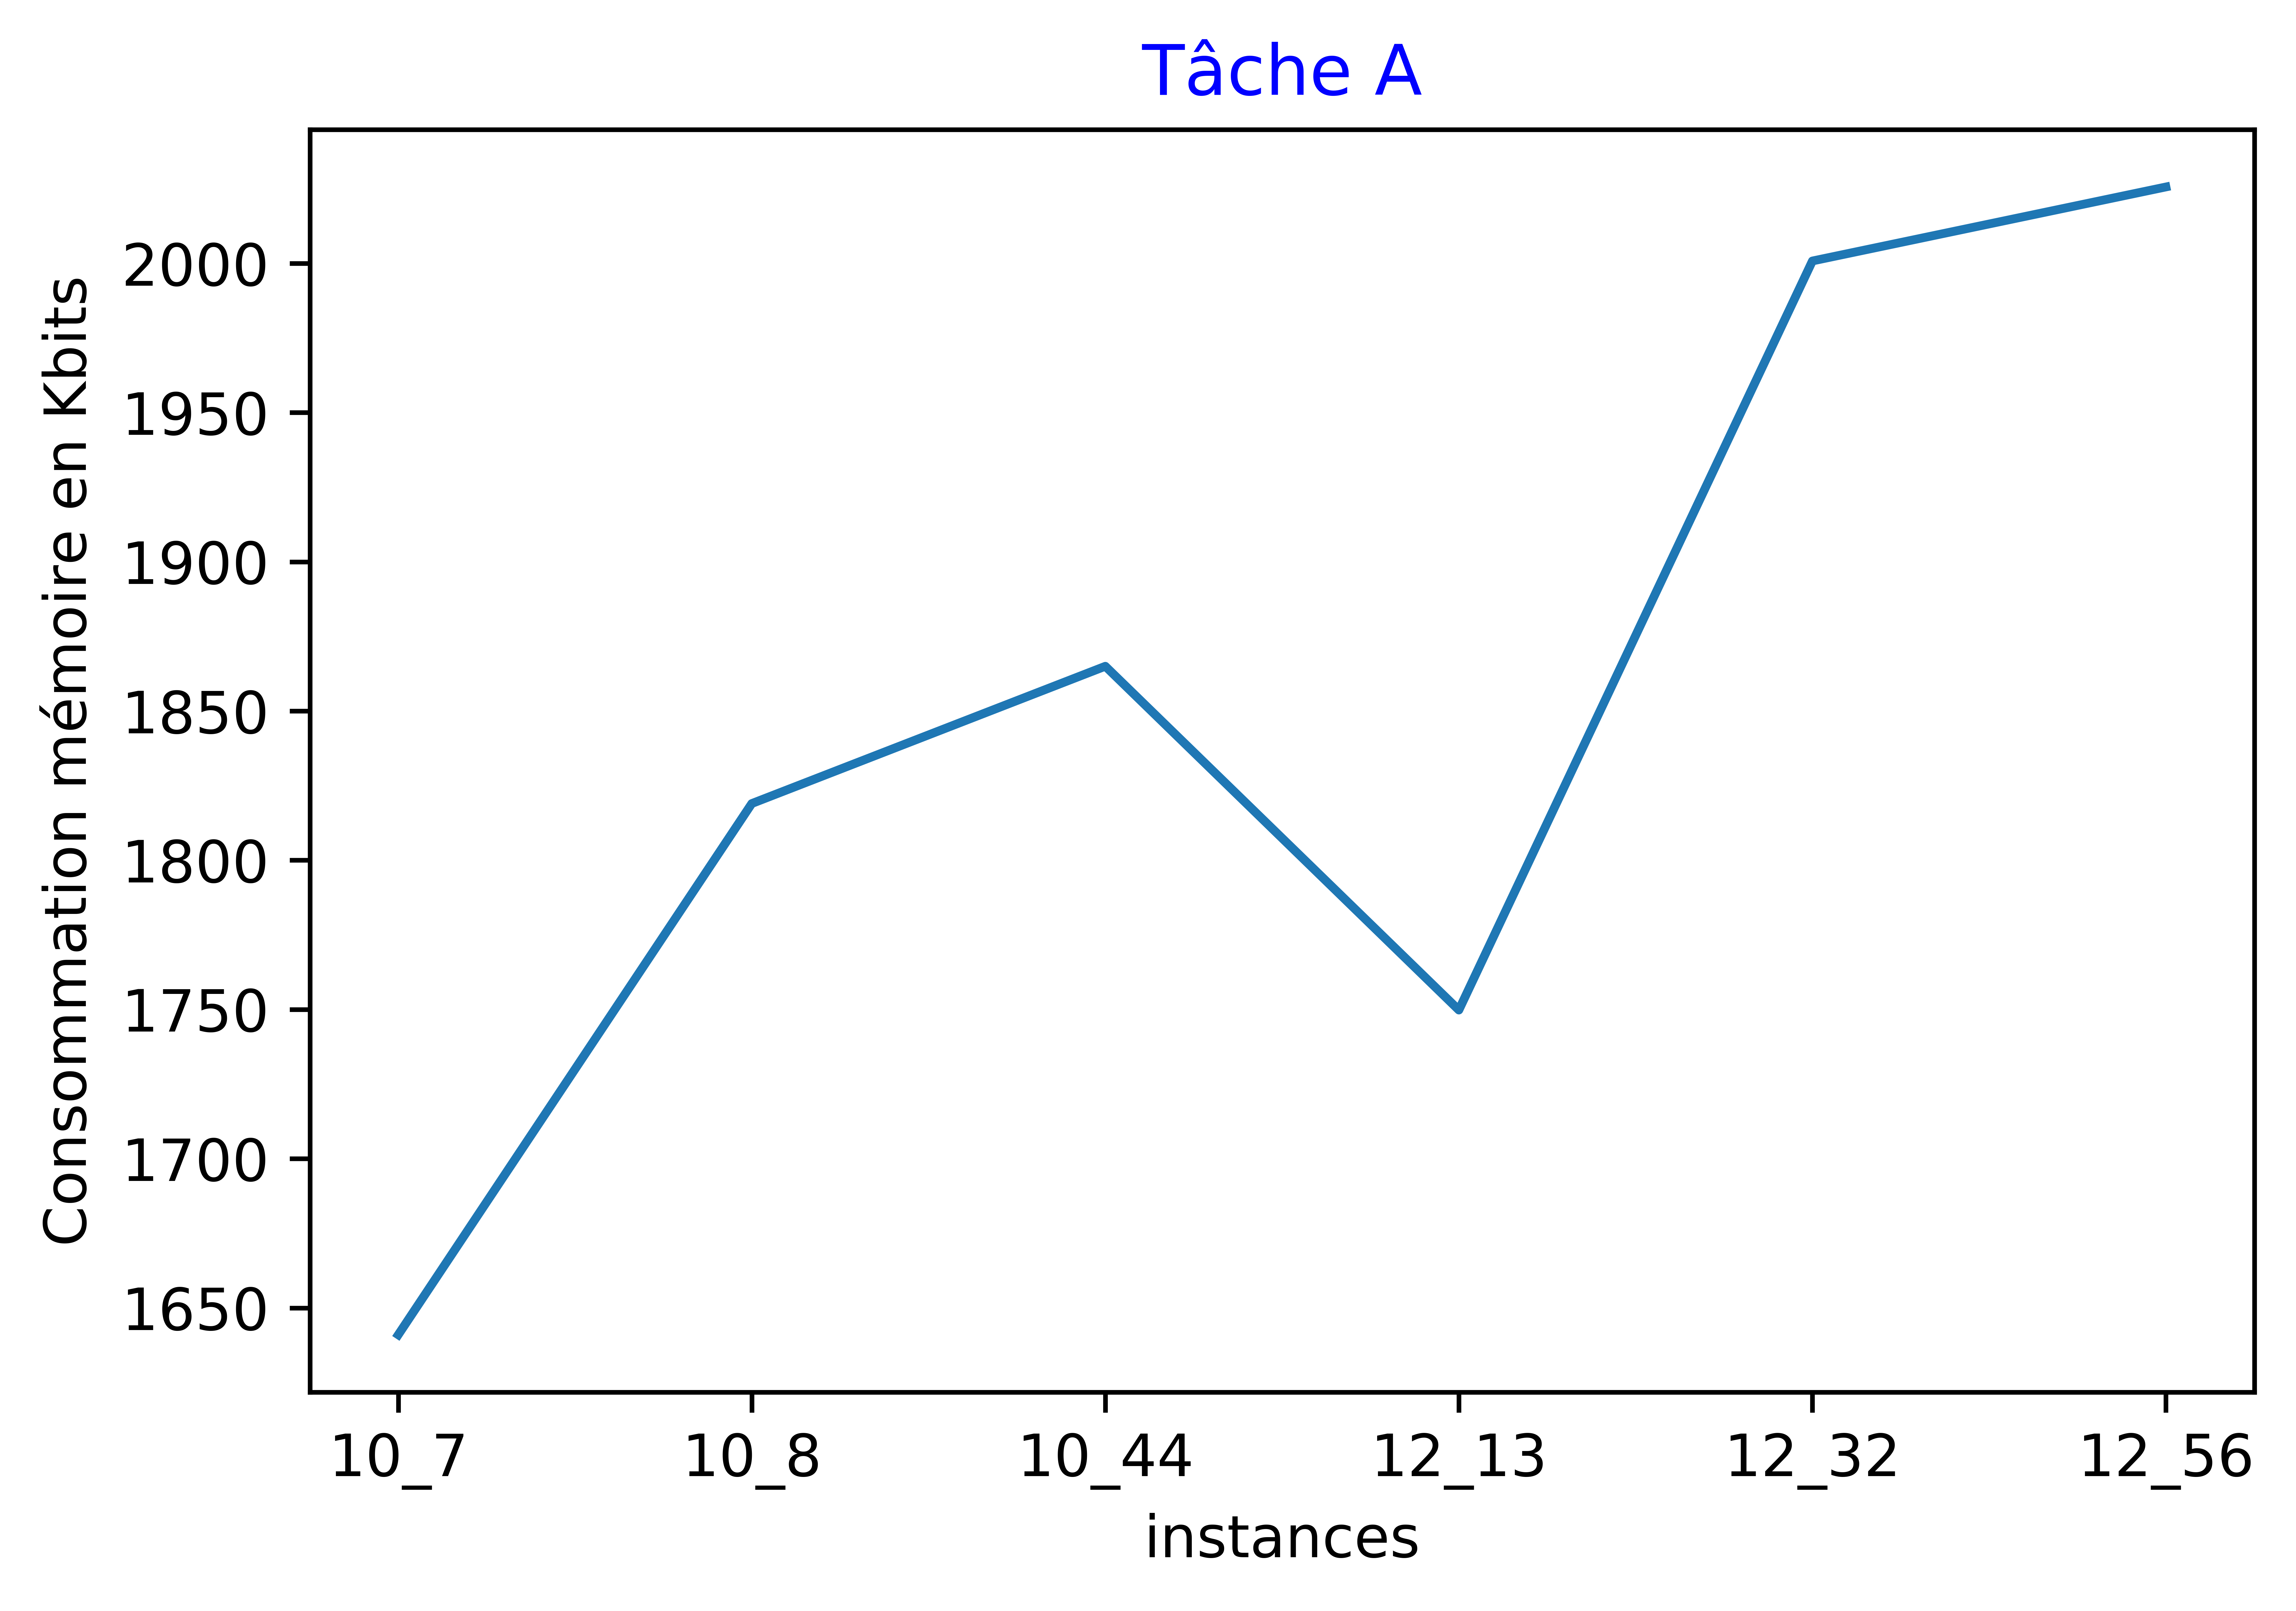
\includegraphics[scale=0.75]{TA2.png}
\end{center}
Il ne nous a été possible de tester que peu d'instances en raison de la complexité trop importante de la fonction. Les données recueillies ayant permis la réalisation du graphe précédent ne sont donc pas suffisantes pour avoir une estimation correcte. Au delà de $Inst\_0000013\_89.adn$, le système stoppe le programme en raison d'une consommation mémoire trop importante.\\
Cependant, sachant qu'en python un $int$ est codé sur $16$ bits, et si l'on ne considère que les paramètres ($i,j,c \text{ et } dist$) dont la valeur évolue pour les fonctions étudiées, on peut écrire que l'on a : $4\times 16 \times \mathcal{O}(n!) \text{ bits}$ consommés, soit une complexité spatiale exponentielle. 
%SUITE analyse consommation mémoire


\section{Programmation dynamique}
\subsection{Calcul de la distance d'édition par programmation dynamique}

\subsubsection{Question 7}
Soit $(\overline{u},\overline{v})$ un alignement de ($x_{\left[ 1 \dots i \right ]},y_{[\left [ 1 \dots j \right ]}$) de longueur $l$.\\ 
Si $\overline{u_{l}}=-$ alors $\overline{v_{l}}$ est un élément de l'alphabet $\Sigma$ tel que $\overline{v_{l}} \in \{ A,T,C,G \}$.\\
Si $\overline{v_{l}}=-$ alors $\overline{u_{l}}$ est un élément de l'alphabet $\Sigma$.\\
Si $\overline{u_{l}}\neq-$ et $\overline{v_{l}}\neq-$, alors ils peuvent soit :
\begin{itemize}
\item correspondre au même caractère.
\item être deux caractères appartenants à une paire concordante.
\item être deux caractères appartenants à une paire non concordante.
\end{itemize}

\subsubsection{Question 8}
Si $\overline{u_{l}}=-$ alors : $C(\overline{u},\overline{v})=C(\overline{u}_{\left [ 1 \dots l-1 \right ]},\overline{v}_{\left [ 1 \dots l-1 \right ]})+c_{ins}$\\
Si $\overline{v_{l}}=-$ alors : $C(\overline{u},\overline{v})=C(\overline{u}_{\left [ 1 \dots l-1 \right ]},\overline{v}_{\left [ 1 \dots l-1 \right ]})+c_{del}$\\
Si $\overline{v_{l}}\neq-$ et $\overline{u_{l}}\neq-$ alors : $C(\overline{u},\overline{v})=C(\overline{u}_{\left [ 1 \dots l-1 \right ]},\overline{v}_{\left [ 1 \dots l-1 \right ]})+c_{sub}(\overline{u}_{l},\overline{v}_{l})$

\subsubsection{Question 9}
Pour $i \in \left [1...n\right]$ et $j \in \left[1...m\right]$, on peut en déduire l'expression de $D(i,j)$ à partir des valeurs de $D$ à des rangs plus petits :  
$$D(i,j)=\min\{D(i',j')+c_{sub}(i,j),D(i,j')+c_{del},D(i',j)+c_{ins}\}$$
On divise le problème en sous-problèmes dont les résolutions successives permettent d'obtenir en fin d'éxecution la solution au problème de départ.
En exprimant $D(i,j)$ en fonction de trois sous-problèmes plus petits qui sont $D(i',j'), D(i,j') \text{ et } D(i',j)$ (réalisation d'une substitution, d'une insertion ou d'une délétion en vue d'arriver à un alignement optimal) dont nous calculons les valeurs puis choisissons  celui dont la distance d'édition est minimale, nous remplissons un tableau à $n$ lignes et $m$ colonnes dont chaque case contient la solution au sous-problème considéré.\\
%Suite underlying dag
La structure de cette méthode de résolution peut aussi être vue comme un graphe orienté acyclique où chaque noeud représente un sous-problème (soit une case du tableau) et chaque arc, une contrainte de précédence sur l'ordre dans lequel les problèmes sont résolus. Si l'on passe de la case $(i-1,j-1)$ à la case $(i,j)$ on réalise une subtitution ou un match. Si l'on passe de la case $(i-1,j)$ à la case $(i,j)$, on réalise une délétion et si l'on va de la case $(i,j-1)$ à la case $(i,j)$, on procède à une insertion.

\subsubsection{Question 10}
Pour le cas de base $i=0$ et $j=0$, on aura $D(0,0)=0$, car considère deux mots vides $\epsilon$. La distance d'édition est donc nulle et il n'y a aucun coût à prendre en compte.
\subsubsection{Question 11}
Pour les deux autres cas de base :
\begin{itemize}
\item Pour $i \in \left[1...n\right]$, on a donc : $D(i,0)=i\times 2$\\
Cela correspond au cas où l'on calcule la distance d'édition entre le préfixe de taille 0 de $y$ et le préfixe $x$, de taille $i$. Ceci nécessite l'ajout de $i$ gaps en $y$, ce qui correspond à réaliser $i$ délétions soit un coût de $i\times c_{del}$ .
\item Pour $j \in \left[1...m\right]$, on a donc : $D(0,j)=j\times 2$\\
Cela correspond au cas où l'on calcule la distance d'édition entre le préfixe de taille 0 de $x$ et le préfixe de $y$, de taille $j$. Ceci se fait en ajoutant $j$ gaps en $x$, ce qui correspond à $j$ insertions soit un coût de : $j\times c_{ins}$ .
\end{itemize}


\subsubsection{Question 12}
\begin{algorithm}[H]
\SetAlgoLined
\KwData{$x$ et $y$ deux mots de tailles $n$ et $m$ tels que $(x,y) \in \Sigma^{*} \times \Sigma^{*}$}
\KwResult{La distance d'édition entre ces deux mots tout en remplissant le tableau $T$ }
Initialisation du tableau $T$ de taille $(|x|+1)\times (|y|+1)$ \;
 \For{$i \in \left[0...n+1\right]$}{
  $T\left[i\right]\left[0\right]=i\times2$\;
  }
  \For{$j \in \left[1...m+1\right]$}{
  $T\left[0\right]\left[j\right]=j\times2$\;
  }
  \For{$i \in \left[1...n+1\right]$}{
	\For{$j \in \left[1...m+1\right]$}{
		$T\left[i\right]\left[j\right]=\min{(T\left[i-1\right]\left[j\right]+c_{del},T\left[i\right]\left[j-1\right]+c_{ins},T\left[i-1\right]\left[j-1\right]+c_{sub}(x\left[i\right],y\left[j\right])}$\;
 	}
}
Return $T\left[n\right]\left[m\right]$
 \caption{DIST\_1}
\end{algorithm}

\subsubsection{Question 13}
L'éxecution de cet algorithme consiste à remplir un tableau de n lignes et m colonnes, ce qui revient donc à une complexité spatiale de $\Theta(nm)$. ($\Theta(nm) \times 16$ bits étant donné que chaque case contient un entier).
\subsubsection{Question 14}
Sachant que le même nombre d'opérations est réalisé à chaque calcul et en supposant que leur éxecution se fait en temps constant, on peut en déduire que la complexité temporelle est elle aussi en $\Theta(nm)$ car DIST\_1 calcule $nm$ valeurs pour résoudre les sous-problèmes considérés.
\subsection{Calcul d'un alignement optimal par programmation dynamique}


\subsubsection{Question 15}
Soit $(i,j) \in \left[1...n\right] \times \left[1...m\right]$, on montre que : si $j>0$ et $D(i,j)=D(i,j-1)+c_{ins}$, alors $\forall (\overline{s},\overline{t}) \in Al^{*}(i,j-1)$, $(\overline{s}\cdot -,\overline{t} \cdot y_{j}) \in Al^{*}(i,j)$. Par l'absurde, si  $j>0$ et $D(i,j)=D(i,j-1)+c_{ins}$, alors $\exists (\overline{s},\overline{t}) \in Al^{*}(i,j-1),\ (\overline{s}\cdot -, \overline{t} \cdot y_{j}) \notin Al^{*}(i,j)$. Dans ce cas, la distance d'édition de $(\overline{s}\cdot -, \overline{t} \cdot y_{j})$ est supérieure à n'importe quel alignement de $Al^{*}(i,j)$. Réaliser une insertion n'est donc pas le meilleur choix pour résoudre le sous-problème (i,j) et une autre opération aurait dû être effectuée. Contradiciton avec le fait que $D(i,j)=D(i,j-1)+c_{ins}$.
Les trois cas présentés permettent de retrouver un alignement optimal possible en remontant de la dernière case du tableau à la première case en respectant les contraintes de précédence à chaque saut de case. Ces contraintes sont déduites des valeurs des cases du tableau $T$ calculées par $DIST\_1$.
\subsubsection{Question 16}
\begin{algorithm}[H]
\SetAlgoLined
\KwData{$x$ et $y$ deux mots tels que $(x,y) \in \Sigma^{*} \times \Sigma^{*}$ et $T$ un tableau indexé par $\left[1...|x|\right]\times \left[1...|y|\right]$ contenant les valeurs de $D$.}
\KwResult{Un alignement minimal de  $(x,y)$}
$u=\left[\right]$\;
$v=\left[\right]$\;
$i=|x|$\;
$j=|y|$\;
\While{$i>0$ and $j>0$}{
	\If{$T\left[i\right]\left[j\right]=T\left[i\right]\left[j-1\right]+c_{ins}$}{
		insérer $-$ en tête de u\;
		insérer $y_{j-1}$  en tête de v\;
		$j = j-1$\;
		passer à l'itération suivante (par un continue)\;
	}
	\If{$T\left[i\right]\left[j\right]=T\left[i-1\right]\left[j\right]+c_{del}$}{
		insérer $x_{i-1}$ en tête de u\;
		insérer $-$  en tête de v\;
		$i=i-1$\;
		passer à l'itération suivante (par un continue)\;
	}
	\If{$T\left[i\right]\left[j\right]=T\left[i-1\right]\left[j-1\right]+c_{sub}(x_{i-1},y_{j-1}$}{
		insérer $x_{i-1}$ en tête de u\;
		insérer substitution($y_{i-1},x_{i-1}$) soit $x_{i-1}$  en tête de v\;
		$i=i-1$\;
		$j = j-1$\;
		passer à l'itération suivante (par un continue)\;
	}
}
\While{$i>0$}{
	insérer $x_{i-1}$ en tête de u\;
	insérer $-$  en tête de v\;
	$i=i-1$\;
}
\While{$j>0$}{
	insérer $-$ en tête de u\;
	insérer $y_{j-1}$  en tête de v\;
	$j = j-1$\;	
}
\caption{SOL\_1}
Return u and v\;
\end{algorithm}

\subsubsection{Question 17}
En combinant $SOL\_1$ et $DIST\_1$, on résout le problème $ALI$ avec une complexité temporelle de : $\Theta(nm)+\Theta(n+m) \subset \Theta(nm)$. Soit une complexité totale de $\Theta(nm)$.\\
Avec $\Theta(nm)$ la complexité requise pour remplir le tableau $T$ et $\Theta(n+m)$ la complexité pour effectuer le parcours permettant de retrouver un alignement optimal.

\subsubsection{Question 18}
La complexité spatiale de $SOL\_1$ et $DIST\_1$ combinés est en  $\Theta(nm)$ car il s'agit toujours d'un tableau à remplir pour la fonction $DIST\_1$ et du parcours de ce même tableau, de la dernière case jusqu'à la première en mettant à jour 2 listes dans lesquelles on stocke les résultats temporaires, ce qui ne modifie pas la complexité spatiale induite par  $DIST\_1$.  

\subsubsection{Tâche B}
\underline{Représentation du temps CPU de l'éxecution de PROG\_DYN en fonction des instances testées} (pour des instances nécessitant moins de 10 minutes chacune) :\\
\begin{center}
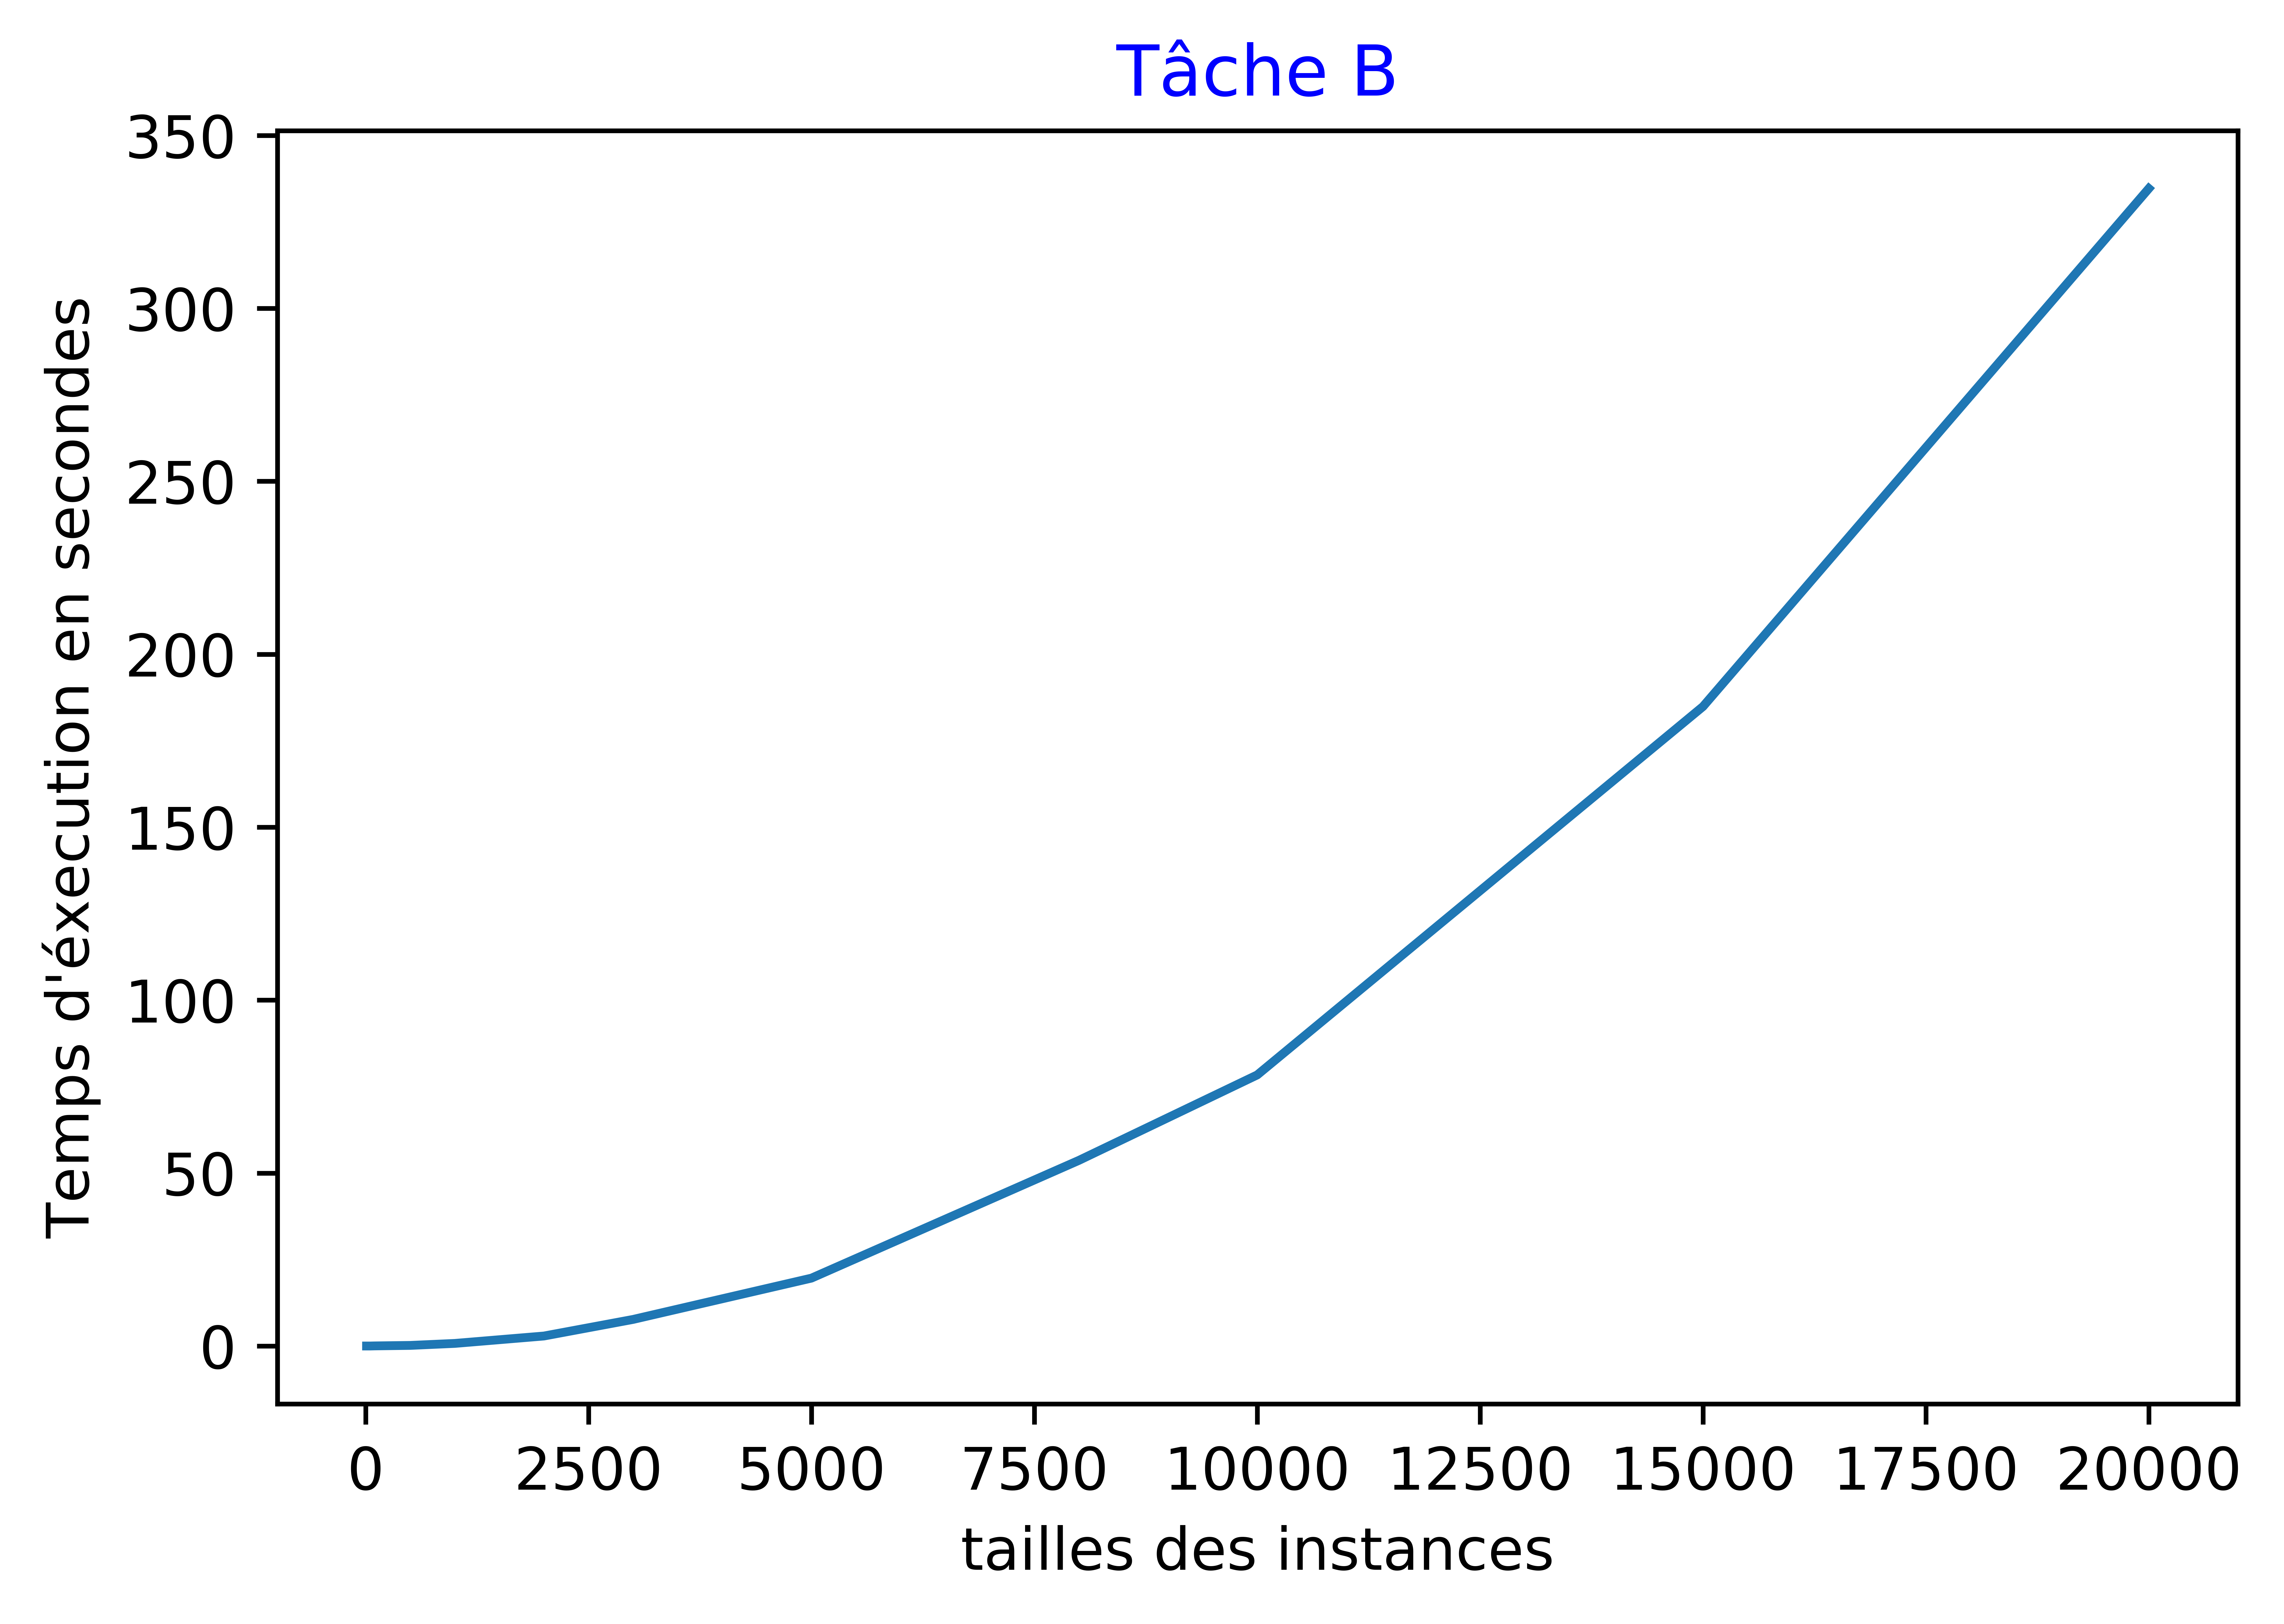
\includegraphics[scale=0.75]{TB.png}
\end{center}
A partir des instances de taille $50\ 000$, l'éxecution se suspend en raison d'une surconsommation de la mémoire utilisée. Il ne nous a donc pas été possible de tester des instances d'une taille supérieure à 20000.\\
La courbe obtenue est en accord avec la complexité théorique. En effet, la courbe montre une évolution similaire à celle d'une fonction polynomiale. Sachant que $n\geq m$, et en supposant que $m\approx \frac{n}{2}$ pour les instances testées, on peut estimer que la courbe se rapproche d'une fonction du type $f(x)=\frac{x^{2}}{2}$.\\
%Représentation de la consommation mémoire de PROG\_DYN en fonction des instances testées :\\
\underline{Estimation de la consommation mémoire pour une instance de très grande taille :}\\
Pour l'instance $Inst0010000\_50.adn$ pour laquelle $|x|=10000$ et $|y|=8882$ et en considérant le fait que chaque caractère est codé sur $8$ bits, on peut calculer que l'on aura : $10000\times 8882 \times 8= 710\ 560\  \text{kbits}$ utilisés. Ce que nous avons vérifié à l'aide d'une mesure expérimentale ayant donné un résultat proche ($\approx 715\ 000 \text{ kbits}$).\\
On remarque une différence importante entre cet algorithme de programmation dynamique et l'algorithme naïf. Les temps d'éxecution pour les instances de petites tailles sont quasiment nuls et rendent la distance d'édition ainsi qu'un alignement optimal. Il est ainsi possible de tester plus d'instances grâce à une meilleure consommation mémoire ainsi qu'un temps de calcul plus rapide. On remarque bien sur le graphe suivant la différence entre la complexité exponentielle du premier algorithme et la complexité polynomiale de $PROG\_DYN$.
\begin{center}
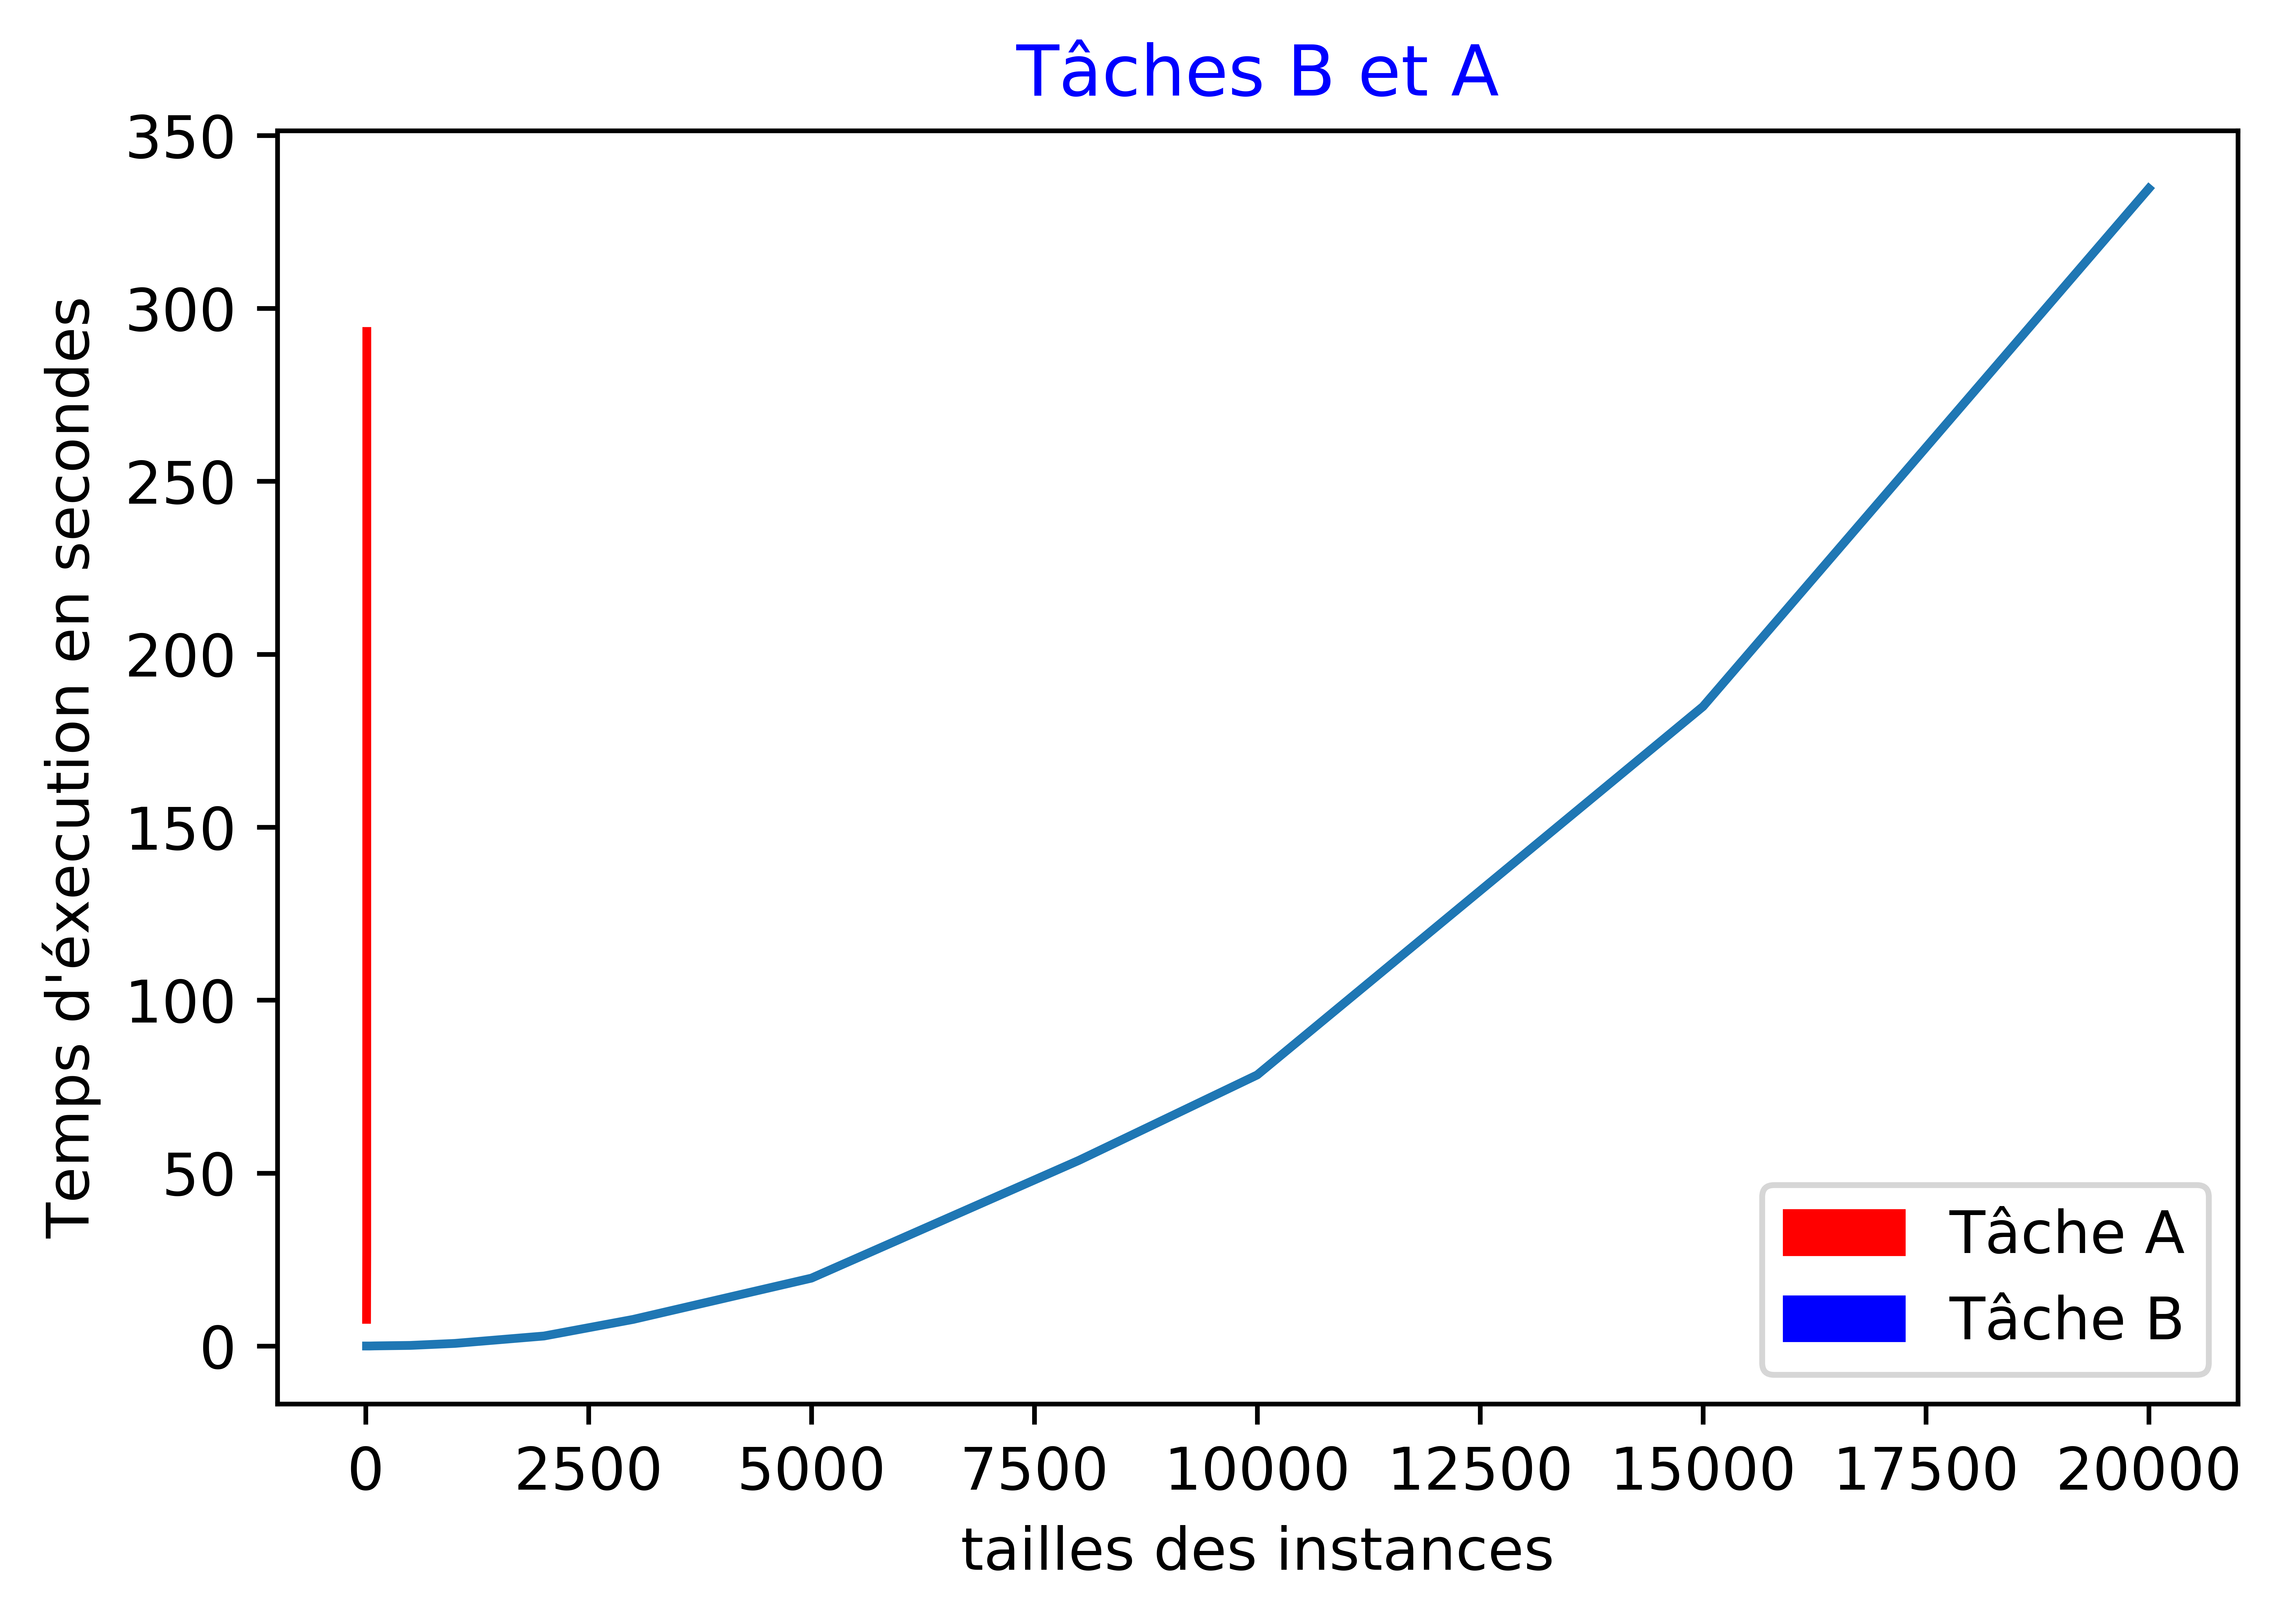
\includegraphics[scale=0.75]{TB22.png}

\end{center}

\subsection{Amélioration de la complexité spatiale du calcul de la distance}

\subsubsection{Question 19}
Lors du calcul de chacune des cases du tableau T (lors de la résolution de chacun des sous-problèmes formant le problème étudié), seules les cases du tableau de la ligne supérieure et de la ligne courante sont nécessaires. A chaque étape, les indices utiles au calcul sont $i$, $i-1$, $j$ ainsi que $j-1$. Seuls les sous-problèmes les plus proches (l'alignement optimal des préfixes considérés) sont nécessaires. Il est donc possible d'arriver à calculer la distance d'édition d'un alignement optimal en ayant recours à beaucoup moins de mémoire que précédemment.

\subsubsection{Question 20}
\begin{algorithm}[H]
\SetAlgoLined
\KwData{$x$ et $y$ deux mots tels que $(x,y) \in \Sigma^{*} \times \Sigma^{*}$}
\KwResult{La distance d'édition entre ces deux mots tout en remplissant le tableau $T$ de dimension $2\times m$}
Initialisation du tableau $T$ de taille $2\times m$ \;
$k=|x|$\;
$cpt = 0$\;
$i = 1$\;
 \For{$j \in \left[1...m\right]$}{
  $T\left[0\right]\left[j\right]=j\times2$\;
  }
  $T\left[1\right]\left[0\right]=2$\;
  \While{cpt<k}{
  	\For{$j \in \left[1...m\right]$}{
  	$T\left[i\right]\left[j\right]=\min{(T\left[(i-1)\%2\right]\left[j\right]+c_{del},T\left[i\right]\left[j-1\right]+c_{ins},T\left[(i-1)\%2\right]\left[j-1\right]+c_{sub}(x_{cpt},y_{j-1})}$\;
  	}
	$i=(i+1)\%2$\;
	$T\left[i\right]\left[0\right]=T\left[(i-1)\%2\right]\left[0\right]+2$\;
	$cpt=cpt+1$\;
}
	\If{k\%2=0}{
		Return $T\left[0\right]\left[m\right]$
}
Return $T\left[1\right]\left[m\right]$
 \caption{DIST\_2}
\end{algorithm}

\subsubsection{Tâche C}
\underline{Représentation du temps CPU de l'éxecution de $DIST\_2$ en fonction des instances testées} (pour des instances nécessitant moins de 10 minutes chacune) :\\
\begin{center}
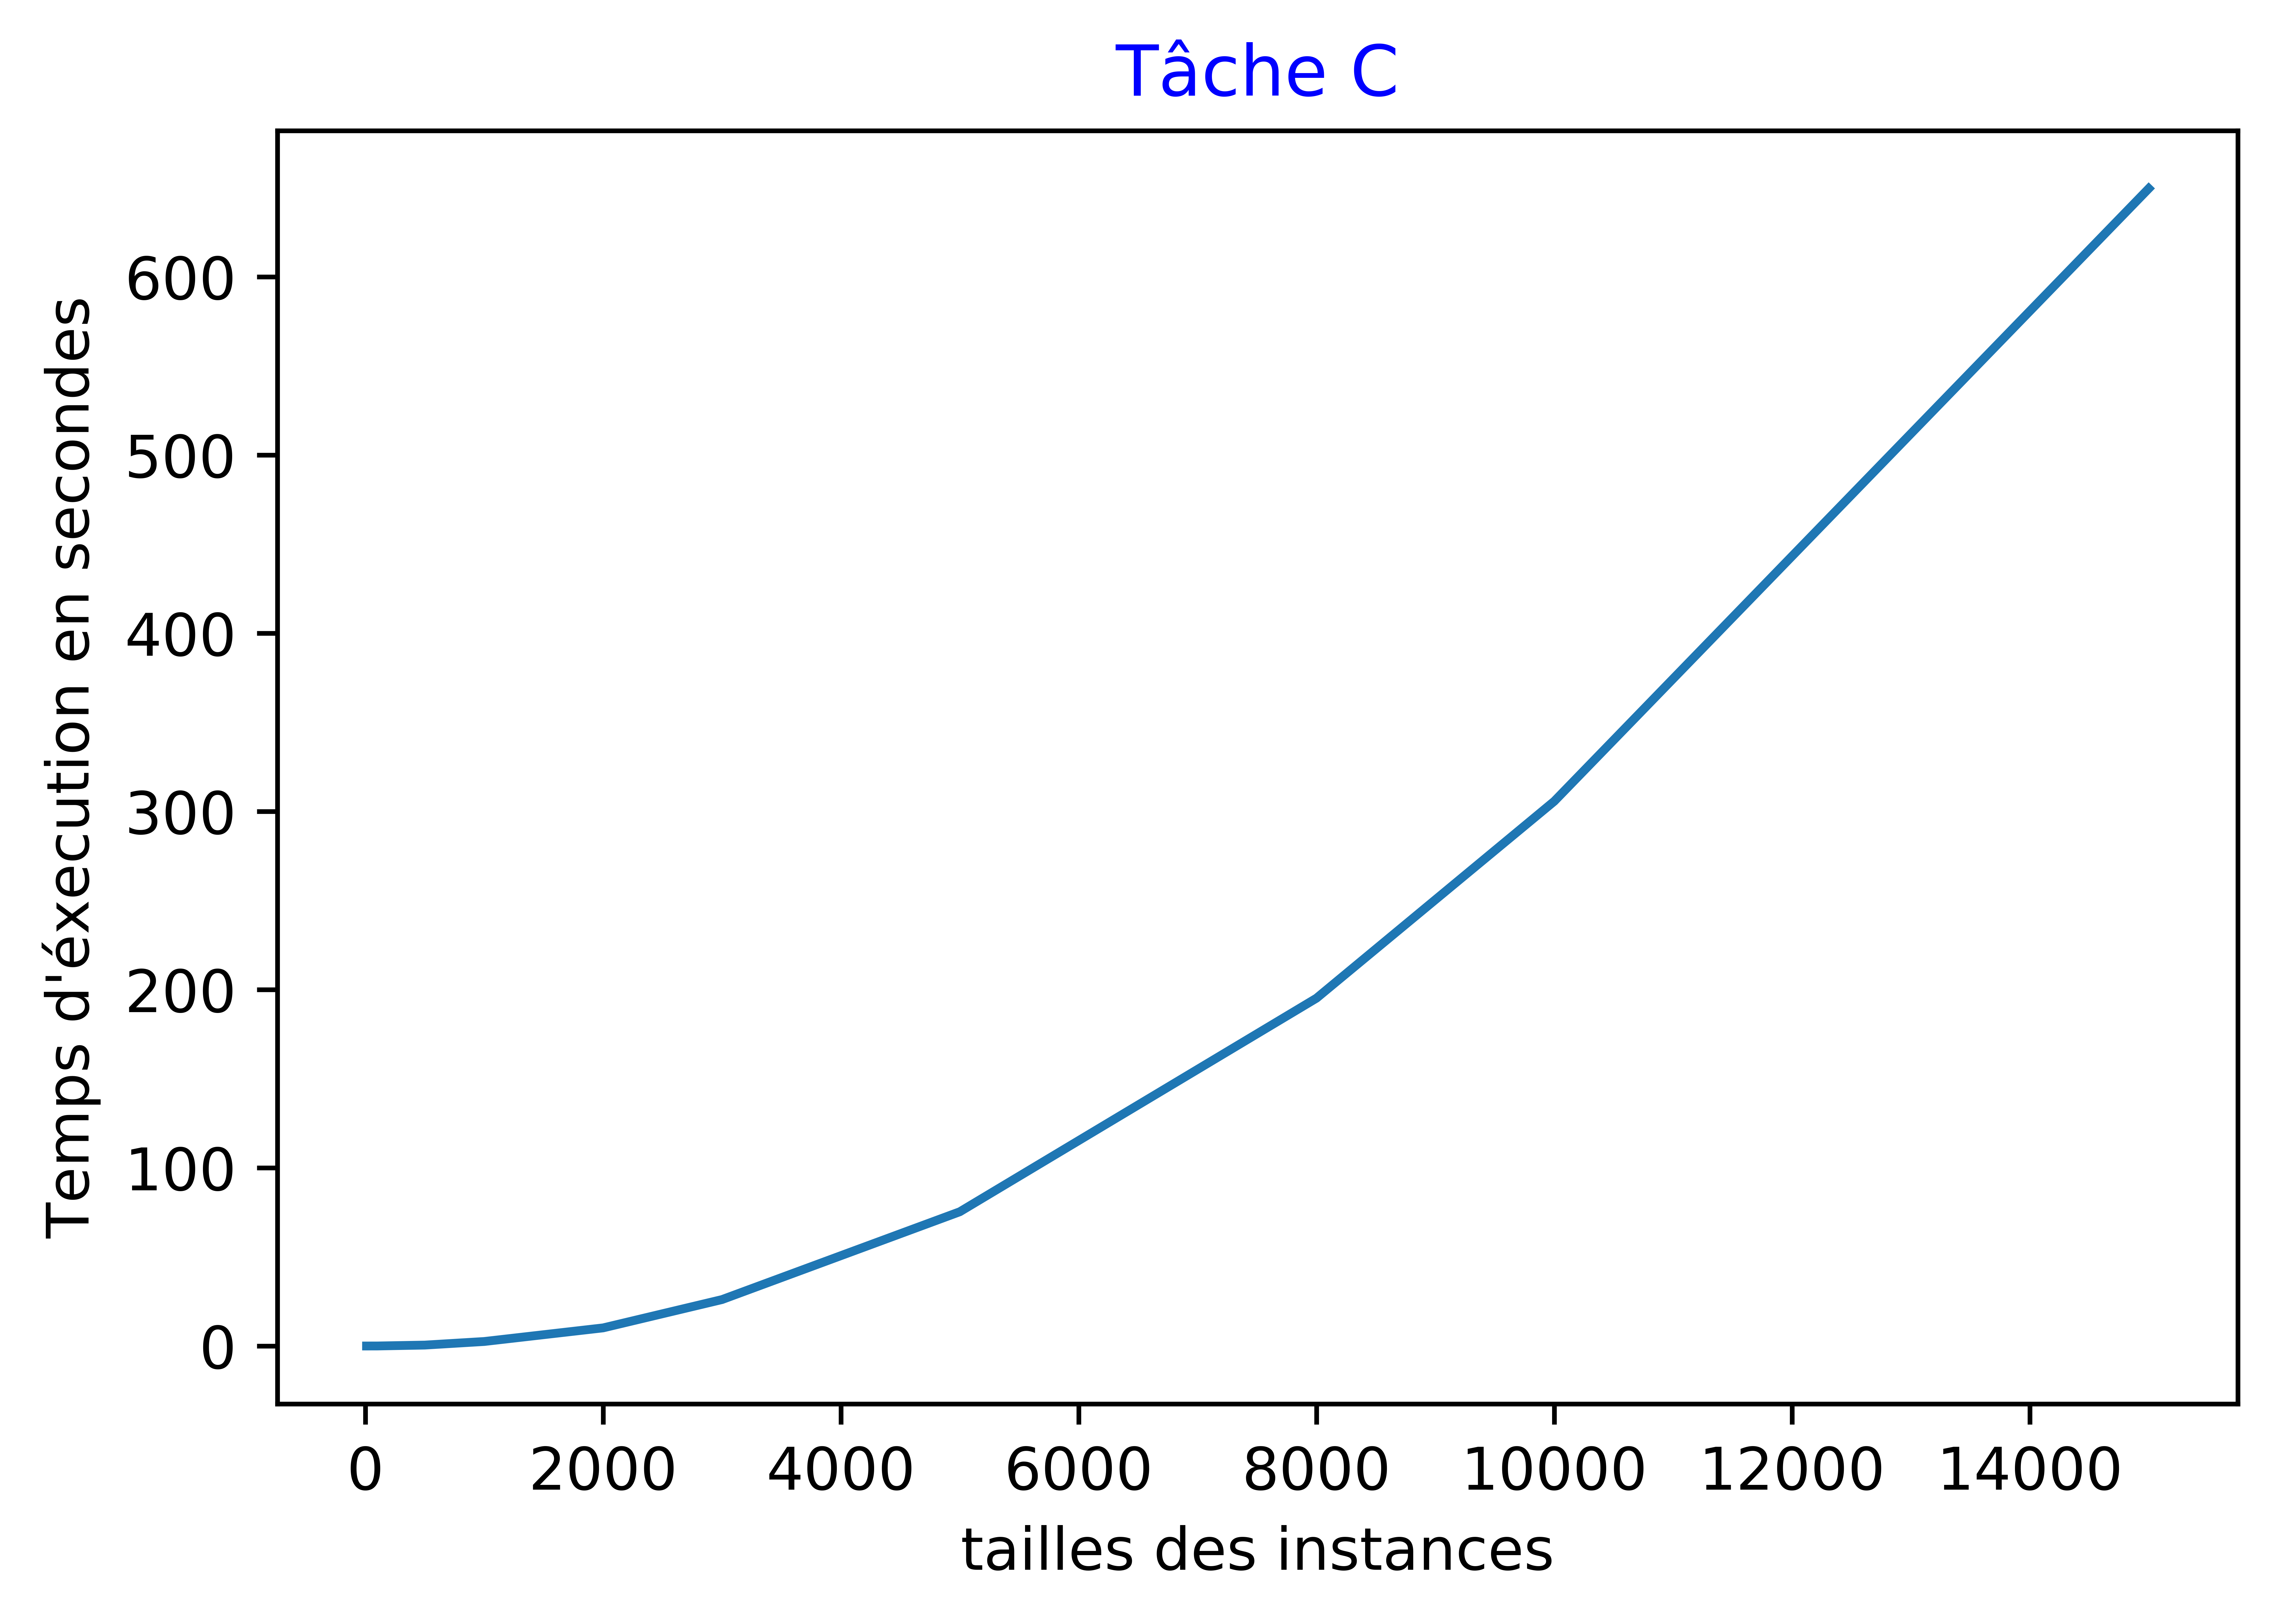
\includegraphics[scale=0.75]{TC.png}
\end{center}
On observe que la courbe correspond bien à la complexité théorique. En effet, la complexité temporelle ne change pas par rapport à l'ancien algorithme car nous faisons toujours $nm$ calculs. On a donc bien une courbe correspondant à une complexité polynomiale. Cependant, les calculs supplémentaires induits par les calculs d'indices et les modulos, augmentent de manière sensible le temps d'éxecution sans toutefois changer le type de complexité.\\
On peut comparer les résultats de $DIST\_2$ avec ceux de $DIST\_1$ :
\begin{center}
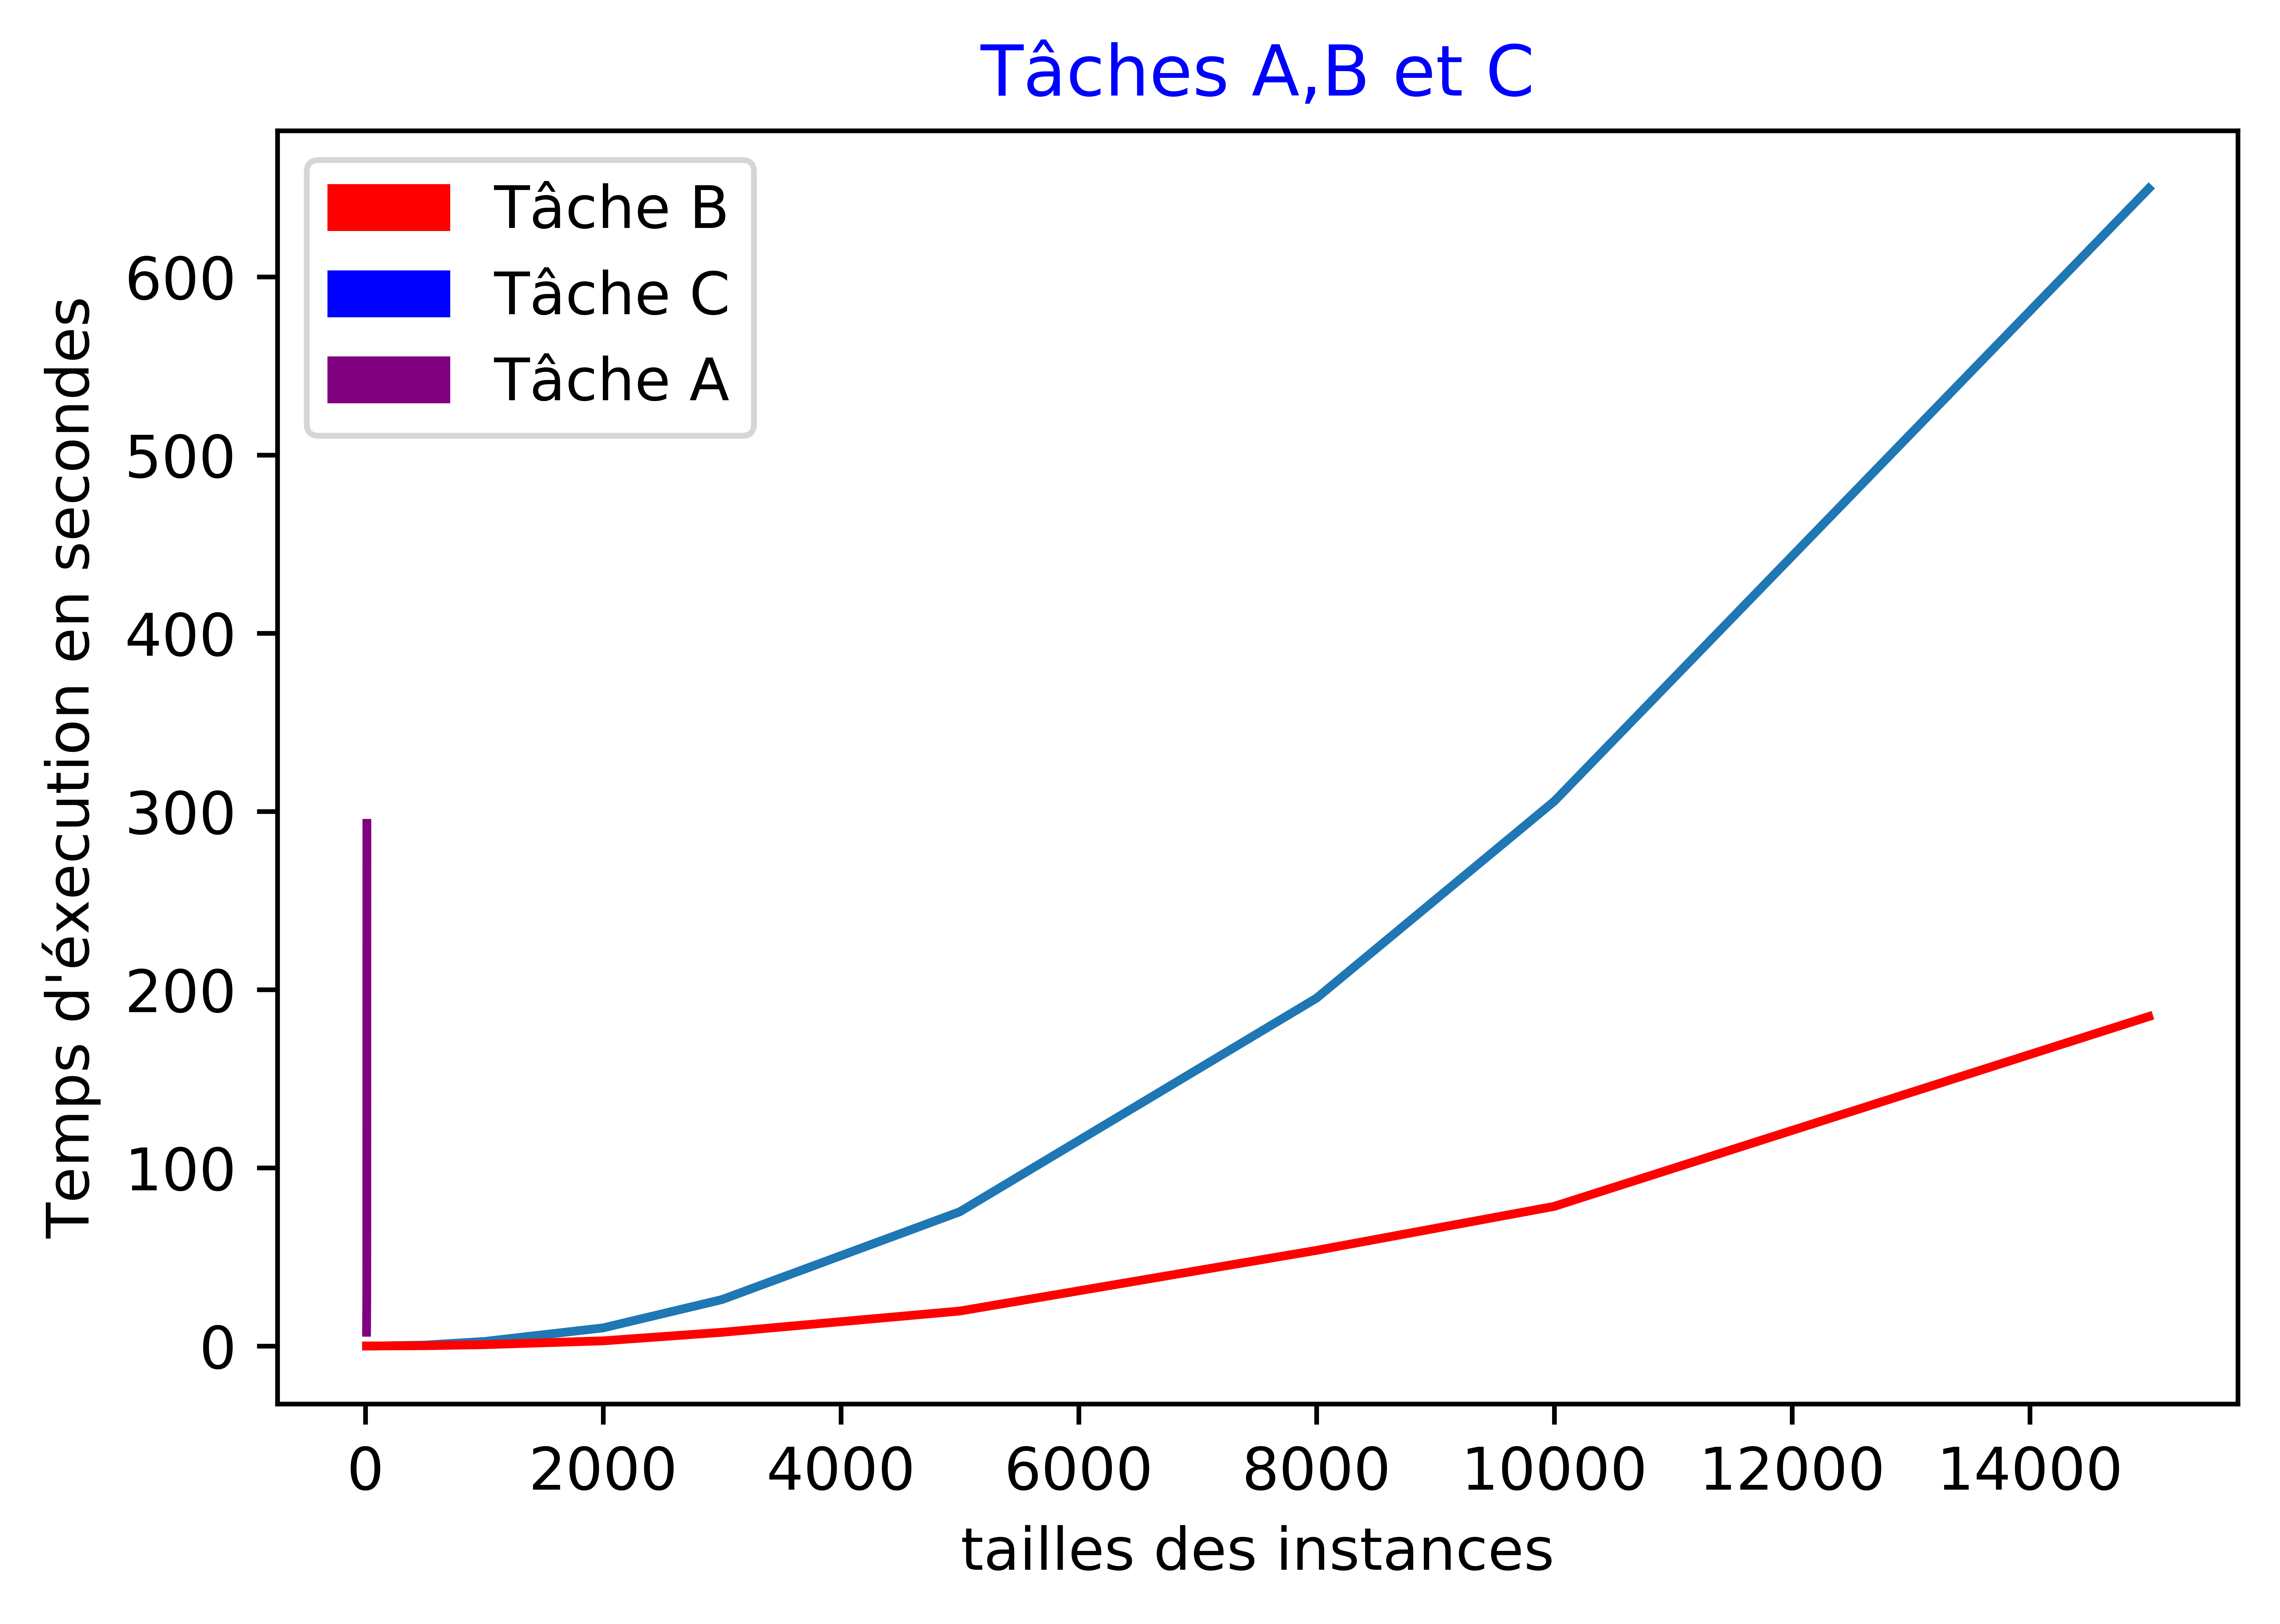
\includegraphics[scale=0.75]{TC2.png}
\end{center}
On voit bien l'augmentation du temps de calcul induite par les calculs d'indices entre la tâche B et la tâche C. Une instance de taille $15000$ est exécutée en environs $200$ secondes pour la tâche B tandis qu'il faut un peu plus de $600$ secondes pour la tâche C. L'évolution en fonction de la taille d'instance reste cependant similaire et est en accord avec celle d'une fonction polynomiale pour les deux algorithmes.
On peut alors estimer la quantité de mémoire utilisée par $DIST\_2$ pour une instance de très grande taille :\\
Pour l'instance $Inst0010000\_50.adn$, sachant qu'un caractère est codé sur $8$ bits et que $|x|=10000$ et $|y|=8882$, on peut calculer que l'on a :\\
$2\times 8882 \times 8=142\ 112$ bits consommés. Ce qui représente une différence importante avec les  $715\ 000 \text{ kbits}$ de la tâche B. $DIST\_2$ a bien une complexité spatiale linéaire en $\Theta(m)$ bien meilleure que la complexité spatiale polynomiale en $\Theta(nm)$ de $DIST\_1$ mais on a en contre partie, une complexité temporelle plus importante.
\section{Amélioration de la complexité spatiale du calcul d'un alignement optimal par la méthode "diviser pour régner"}

\subsubsection{Question 21}
\begin{algorithm}[H]
\SetAlgoLined
\KwData{$k \in \mathbb{N}$ }
\KwResult{Le mot constitué de $k$ gaps}
Return $k \times -$\;
\caption{mot\_gaps}
\end{algorithm}

\subsubsection{Question 22}
\begin{algorithm}[H]
\SetAlgoLined
\KwData{$x$ un mot de longueur $1$ et $y$ un mot non vide de longueur quelconque }
\KwResult{un meilleur alignement parmi ceux possibles pour $(x,y)$}
$i = 0$\;
\While{$i<|y|$}{
	\If{$y_{i}=x$}{
		Return (mot\_gaps($i$)+x+mot\_gaps($|y|-i-1),y$)\;
	}
	$i=i+1$\;
}
$i=0$\;
\While{$i<|y|$}{
	\If{$c_{sub}(x,y_{i})=3$}{
		Return (mot\_gaps($i$)+substitution2($x,y_{i}$)+mot\_gaps($|y|-i-1),y$)\;
	}
	$i=i+1$\;
}
\If{$i=|y|$}{
	Return (mot\_gaps($i-1$)+substitution2($x,y_{i-1}$),$y$)\;
}
\caption{align\_lettres\_mot}
\end{algorithm}
substitution2($a,b$) étant une fonction qui renvoie le caractère $a$ à chaque appel pour réaliser la substitution de $b$ par $a$. \\

\subsubsection{Question 23}
Un alignement optimal ($\overline{s},\overline{t}$) de ($x^{1},y^{1}$) est :
\begin{center}
$x^{1}=BAL$ et $y^{1}=RO$\\
\rule{0.4\textwidth}{.4pt}\\
\begin{tabular}{llll}
$\overline{s}$ :&B&A&L\\
$\overline{t}$ :&B&A&-\\
\end{tabular}\\
\rule{0.4\textwidth}{.4pt}
\end{center}
Avec un coût de $13$.\\
Un alignement optimal ($\overline{u},\overline{v}$) de ($x^{2},y^{2}$) est :
\begin{center}
$x^{2}=LON$ et $y^{2}=ND$\\
\rule{0.4\textwidth}{.4pt}\\
\begin{tabular}{lllll}
$\overline{u}$ :&L&O&N&-\\
$\overline{v}$ :&-&-&N&D\\
\end{tabular}\\
\rule{0.4\textwidth}{.4pt}
\end{center}
Avec un coût de $9$.\\

$(\overline{s} \cdot \overline{u},\overline{t} \cdot \overline{v})$ n'est pas un alignement optimal de $(x,y)$ car on obtiendrait:
\begin{center}
$x=BALLON$ et $y=ROND$\\
\rule{0.4\textwidth}{.4pt}\\
\begin{tabular}{llllllll}
$\overline{u}$ :&B&A&L&L&O&N&-\\
$\overline{v}$ :&B&A&-&-&-&N&D\\
\end{tabular}\\
\rule{0.4\textwidth}{.4pt}
\end{center}
Avec un coût total de $22$.\\

Alors qu'il est possible d'obtenir :
 \begin{center}
\rule{0.4\textwidth}{.4pt}\\
\begin{tabular}{llllllll}
$\overline{u}$ :&B&A&L&L&O&N&-\\
$\overline{v}$ :&B&-&-&-&O&N&D\\
\end{tabular}\\
\rule{0.4\textwidth}{.4pt}
\end{center}
Avec un coût total de $17<20$. L'alignement précédent n'est donc pas optimal.\\

\subsubsection{Question 24}
\begin{algorithm}[H]
\SetAlgoLined
\KwData{$x$ et $y$ deux mots.\\$u$ et $v$ deux paramètres servant à stocker les alignements optimaux temporaires
                et qui contiendront en fin d'éxecution les alignements optimaux de $x$ et $y$}
\KwResult{$(u,v)$ l'alignement optimal calculé pour $(x,y)$}
$n=|x|$ \;
$m=|y|$ \;
$i=\left \lfloor \frac{n}{2} \right \rfloor$ \;
\uIf{$m=0 \text{ et } n\neq 0$}{
	ajouter x à u \;
	ajouter $n$ gaps à v \;
}
\uElseIf{$n=0 \text{ et } m \neq 0$}{
	ajouter $m$ gaps à $u$ \;
	ajouter y à $v$ \;	
}
\uElseIf{$n=1 \text{ et } m \geq 1$}{
	ajouter à u le premier élément du tuple résultat de align\_lettre\_mot($x,y$) \;
	ajouter à v le second élément du tuple résultat de align\_lettre\_mot($x,y$) \;
}
\uElseIf{$n>1 \text{ et } m \geq 1$}{
	j=coupure($x,y$) \;
	SOL\_2($x\left[:i\right],y\left[:j\right],u,v$) \;
	SOL\_2($x\left[i:\right],y\left[j:\right],u,v$) \;
}
Return $(u,v)$ \;
\caption{SOL\_2}
\end{algorithm}
Les sous-mots sont indexés comme des sous-tableaux en python au sein des appels récursifs à $SOL\_2$.

\subsubsection{Question 25}
\begin{algorithm}[H]
\SetAlgoLined
\KwData{$x$ et $y$ deux mots.}
\KwResult{l'indice $j^{*}$ permettant de réaliser la coupure de $(x,y)$ sachant que $i^{*}=\frac{|x|}{2}$}
Initialisation de deux tableaux $T$ et $I$ de dimensions $2 \times m$ \;
$k=|x|$ \;
$coup=\left \lfloor \frac{k}{2} \right \rfloor$ \;
$cpt=0$ \;
$i=1$ \;
$i2=1$ \;
\For{ $j \in \left[1...m+1\right]$}{
	$T\left[0\right]\left[j\right]=j\times2$ \;
}
$T\left[i\right]\left[0\right]=2$ \;
\For{ $j \in \left[0...m+1\right]$}{
	$I\left[0\right]\left[j\right]=j$ \;
	$I\left[1\right]\left[j\right]=j$ \;
}
\While{$cpt < k $}{
	\For{$j \in \left[1...m+1\right]$}{
  		$T\left[i\right]\left[j\right]=\min{(T\left[(i-1)\%2\right]\left[j\right]+c_{del},T\left[i\right]\left[j-1\right]+c_{ins},T\left[(i-1)\%2\right]\left[j-1\right]+c_{sub}(x_{cpt},y_{j}))}$ \;
		\uIf{$cpt \geq coup$}{
			\uIf{$T\left[i\right]\left[j\right]=T\left[(i-1)\%2\right]\left[j\right]+c_{del}$}{
					$I\left[i2\right]\left[j\right]=I\left[(i2-1)\%2\right]\left[j\right]$ \;
			}
			\uElseIf{$T\left[i\right]\left[j\right]=T\left[i\right]\left[j-1\right]+c_{ins}$}{
				$I\left[i2\right]\left[j\right]=I\left[i2\right]\left[j-1\right]$ \;
			}
			\uElseIf{$T\left[i\right]\left[j\right]=T\left[(i-1)\%2\right]\left[j-1\right]+c_{sub}(x_{cpt},y_{j-1})$}{
				$I\left[i2\right]\left[j\right]=I\left[(i2-1)\%2\right]\left[j-1\right]$ \;
			}
		}
	}
	\uIf{$cpt \geq coup$}{
		$i2=(i2+1)\%2 $\;
	}
	$i=(i+1)\%2$ \;
	$T\left[i\right]\left[0\right]=T\left[(i-1)\%2\right]\left[0\right]+2$ \;
	$cpt=cpt+1$ \;
}
\uIf{$(k-coup)\%2=0$}{
	Return $I\left[0\right]\left[|y|\right]$ \;
}
Return $I\left[1\right]\left[|y|\right]$ \;
\caption{Coupure}
\end{algorithm}

\subsubsection{Question 26}
Lors de l'éxecution de l'algorithme, on a recours aux lignes $i$ et $i-1$ des Tableaux $T$ et $I$ (le tableau $I$ n'étant rempli qu'à partir de la moitié du tableau $T$) , on peut affirmer que la complexité spatiale de $coupure$ est donc en : $$\Theta(4m) \text{ soit une complexité de } \Theta(m)$$

\subsubsection{Question 27}
Dans le pire des cas, si $n=m$ et si l'on a $n-1$ coupures pour le couple de mots considéré, on sera dans le cas où l'arbre des appels récursifs est complet. Sachant qu'il s'agit d'un arbre binaire, il sera donc de hauteur $\log_{2}{(n)}$ et le nombre total d'appels récursifs sera de $2^{\log_{2}{(n)}+1}-1=2n-1$.
A chaque appel récursif engendrant d'autres appels récursifs (donc non résolus par un cas de base), la fonction coupure utilisée a une complexité spatiale en $\Theta(m)$. Une fois l'indice de la coupure $j^{*}$ calculé, la mémoire utilisée par coupure est libérée. Ainsi, $SOL\_2$ a une consommation mémoire en $\Theta(\max(n+m))$, avec toutefois une consommation inférieure à $DIST\_2$ car seule les listes servant à retourner les résultats sont gardées en mémoire du début à la fin de l'éxecution.
%utilisée puis libérée


\subsubsection{Question 28}

$coupure$ réalise toujours $n\times m$ calculs pour déterminer la distance d'édition ainsi que le tableau $I$ donnant les coupures du couple de mot étudié. A partir de  $i^{*}=\frac{|x|}{2}$, le tableau $I$ est aussi mis à jour, ce qui implique des comparaisons supplémentaires. Cependant on peut considérer que ces calculs et ces mises à jour, se font en temps constant et $coupure$ a donc une complexité temporelle en $\Theta(nm)$.


\subsubsection{Tâche D}
\underline{Représentation du temps CPU de l'éxecution de $SOL\_2$ en fonction des instances testées} (pour des instances nécessitant moins de 10 minutes chacune) :\\
On observe sur cette courbe, une évolution comparable à celle d'une fonction polynomiale. La complexité théorique en $\Theta(nm)$ est donc en accord avec la complexité mesurée. En effet, pour $n>1$ et $m\geq 1$, $SOL\_2$ fait appel à $coupure$ qui est en $\Theta(nm)$ et entraîne deux appels récursifs. Si l'on suppose que $coupure$ coupe chaque sous-mot en deux sous-mots de longueurs approximativement égales (ce qui peut amener à une perte de généralité, mais qui est vrai pour certaines instances que nous avons testé) et sachant que $align\_lettres\_mots$ a une complexité en $\Theta(n+m) \sim \Theta(n)$ et que $m\approx \frac{n}{2}$, on peut essayer d'écrire une équation de récurrence: $$T(n)=2T(\left \lfloor \frac{n}{2} \right \rfloor)+\Theta(nm) \sim 2T(\left \lfloor \frac{n}{2} \right \rfloor)+\Theta(n^{2})$$
En appliquant le théorème maître, il est possible de déduire que $SOL\_2$ a une complexité en $\Theta(n^{2})$.
\begin{center}
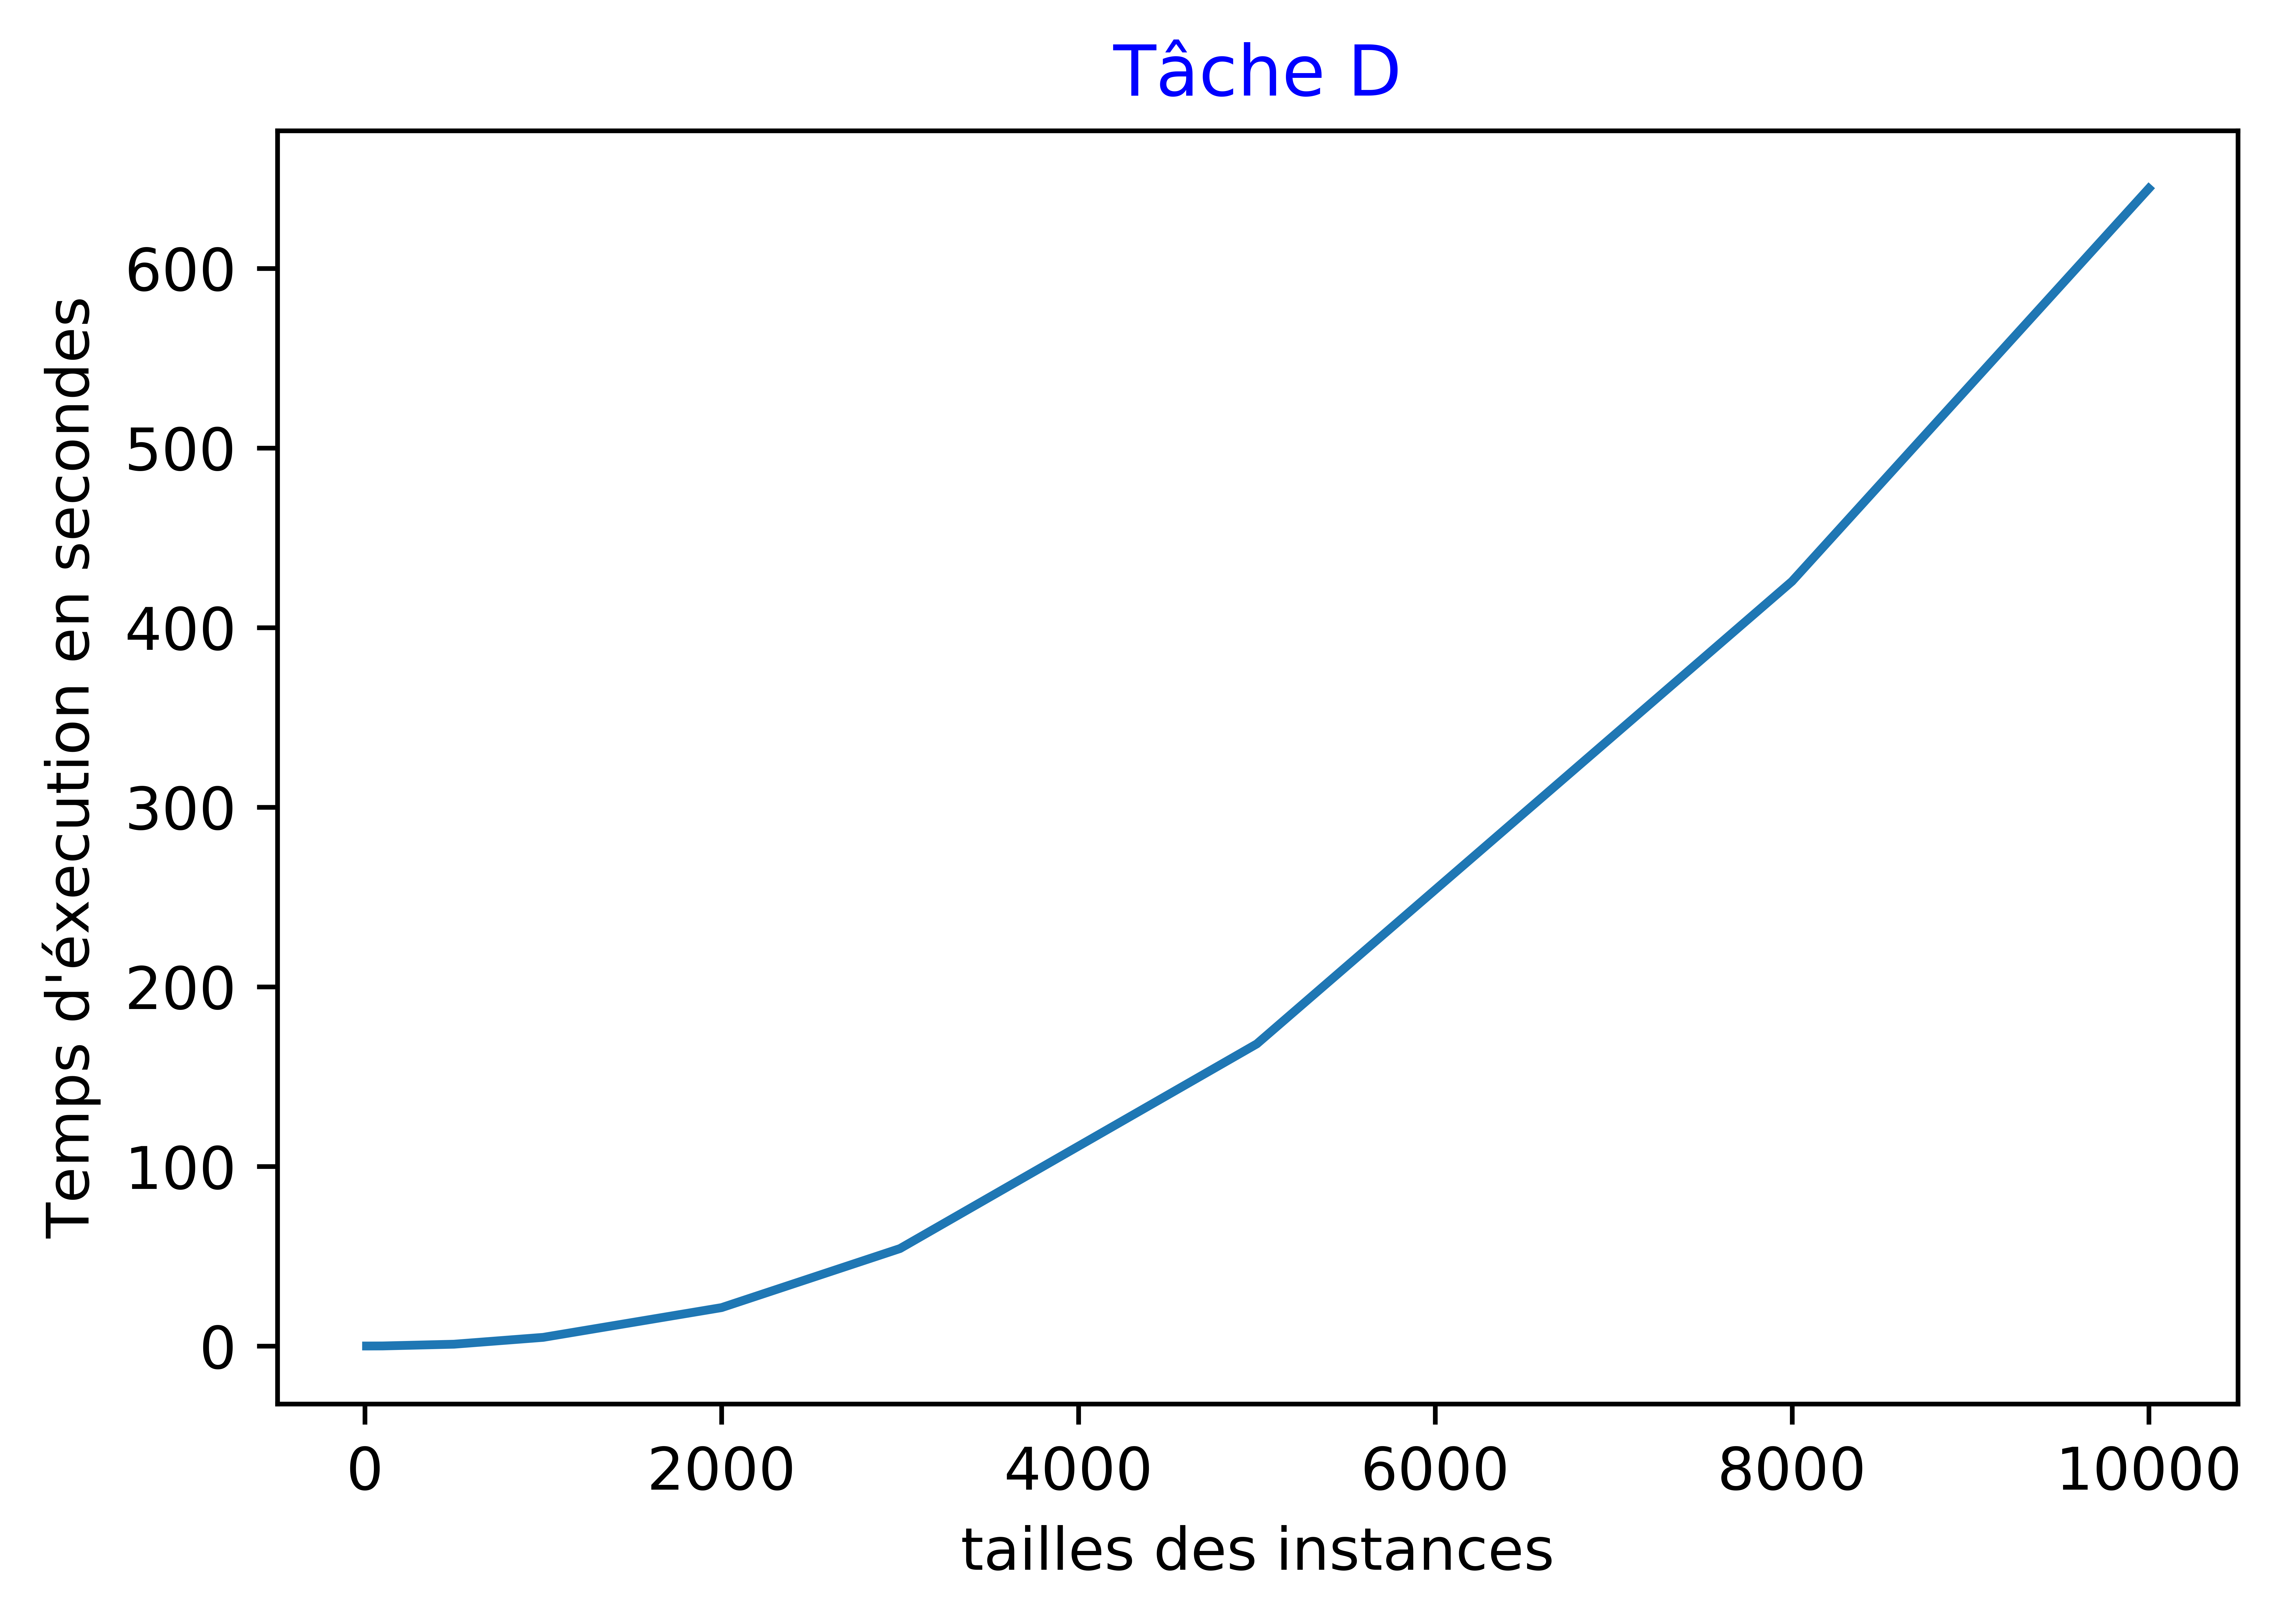
\includegraphics[scale=0.75]{TD.png}
\end{center}
On peut estimer la consommation mémoire de $SOL\_2$, si l'on considère le fait que $coupure$ libère la mémoire à chaque fois qu'elle est appelée, que chaque caractère est codé sur 8 bits et que l'on stocke les résultats dans deux listes dont la taille maximale est de $n+m$, on peut affirmer que l'on a : $8 \times 2 \times (n+m)$ bits consommés.\\
Pour l'instance $Inst\_0001000\_23.adn$ on peut estimer que l'on aura :\\ $8 \times 2 \times (1000+887)=30\ 196$ bits consommés. Notre mesure expérimentale a donné $30.9$ Kbits (pour chacune des mesures, un espace mémoire supplémentaire doit être considéré en raison du fait que l'éxecution a lieu au sein d'un environnement d'éxecution consommant lui aussi de la mémoire d'où les bits en surplus dans les mesures). On en déduit que la complexité spatiale est bien en $\Theta(n+m)$ ce qui est meilleur ques les algorithmes des tâches B et C.

\subsection{Question 29}
\begin{center}
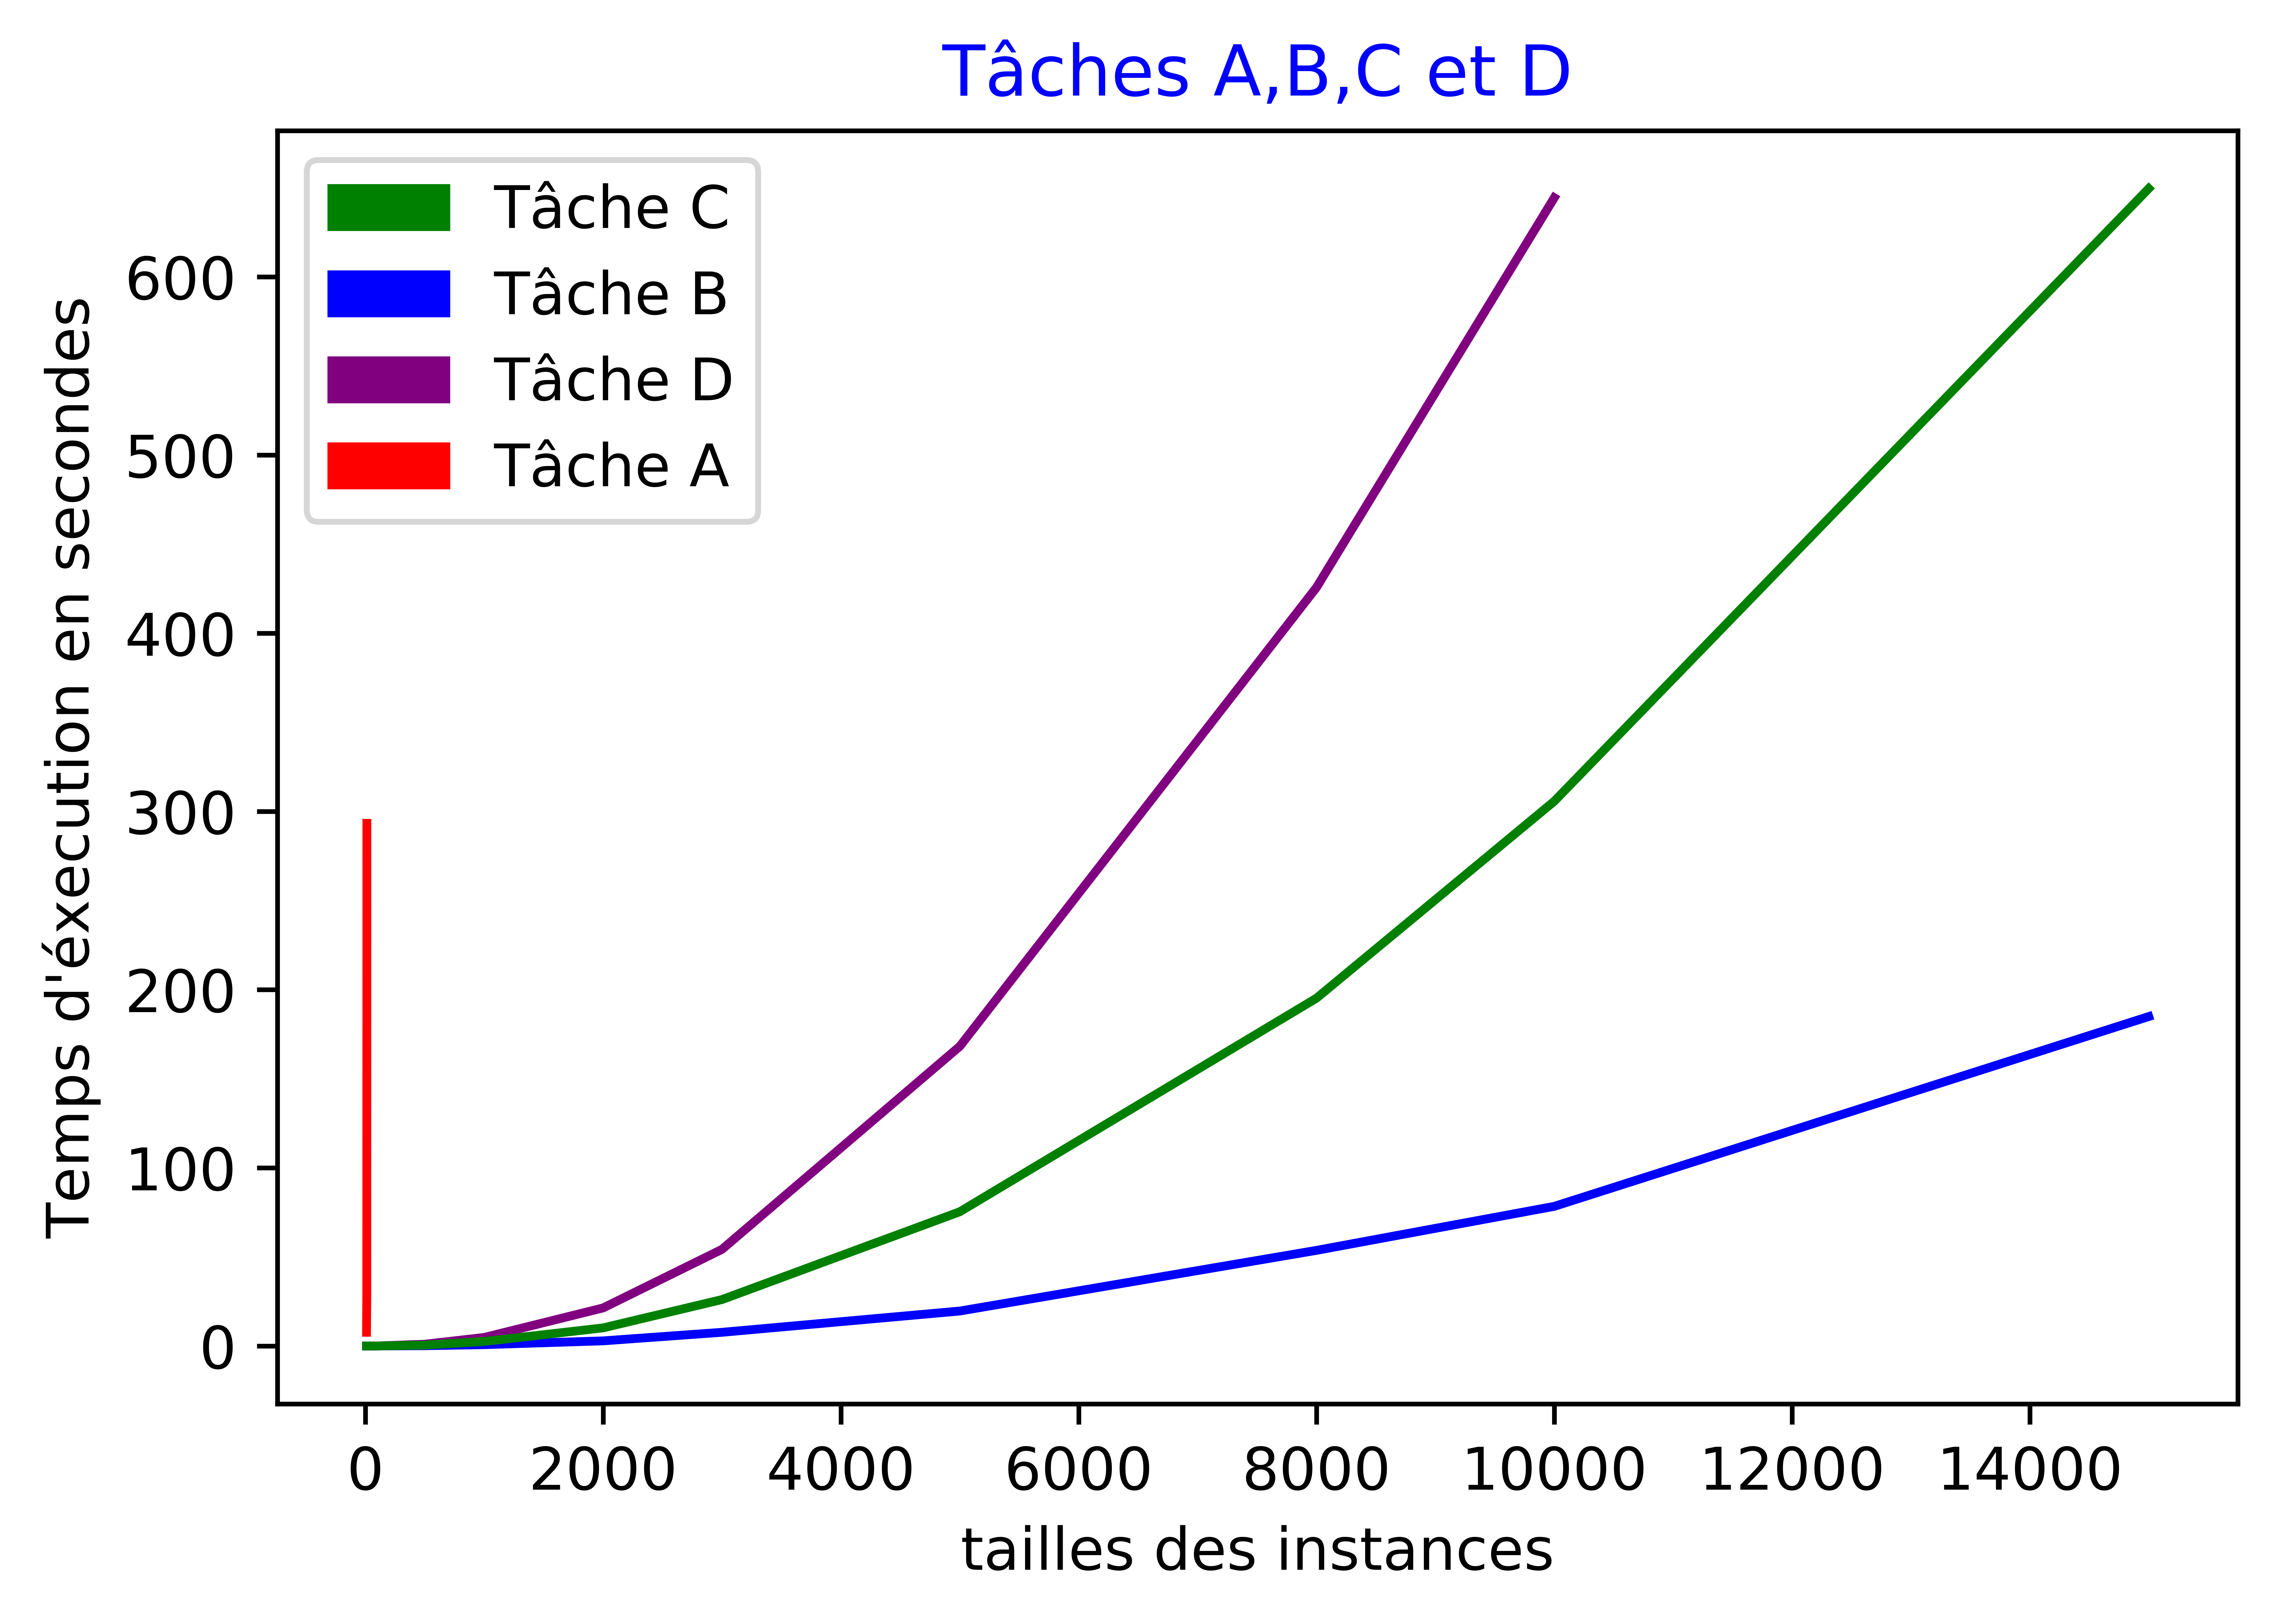
\includegraphics[scale=0.75]{TD2.png}
\end{center}
Lors de la réalisation des tâches B, C et D, nous avons à chaque fois réduit la consommation mémoire nécessaire à la résolution du problème d'alignement des séquences. Nous avons remarqué que l'algorithme de la tâche C consommait effectivement moins de mémoire que celui de la tâche B mais entraînait un temps de calcul plus long. Il était cependant possible d'atteindre la même taille d'instance pour les 2 algorithmes .\\
Pour la tâche D, on remarque clairement sur le graphe comparatif ci-dessus que la complexité temporelle de D (bien qu'étant de même type) est bien supérieure à celle de B et C. Pour les tâches B et C, il nous a été possible de tester des instances ayant une taille maximale de $15\ 000$ tandis que pour la tâche D, on dépasse les $10$ minutes de temps d'éxecution dès une instance de taille $10\ 000$. Il est donc clair qu'en passant à une complexité spatiale moins importante pour la tâche D, nous avons perdu de manière importante en complexité temporelle avec un nombre maximal de $10\ 000$ nucléotides pouvant être testés en un temps raisonnable. Cela peut s'expliquer par le fait que l'utilisation de la fonction coupure calcule plusieurs fois le tableau $T$ donnant les distances d'éditions pour les sous-mots considérés. A chaque coupure, on calcule le tableau $T$ pour le sous-mot que l'on veut couper de manière à obtenir un alignement optimal et il apparait clairement que la tâche D est plus lente par rapport à la tâche C qui elle même est plus lente que la tâche B. Il est donc possible de résoudre ce problème avec une complexité spatiale linéaire mais au détriment de la complexité temporelle.

\end{document}

